\chapter{Belief Change for Horn Formulas}\label{ch:6}

In this chapter we look at revision and update for \emph{Horn formulas},
a type of propositional formulas used to represent facts and rules,
i.e., information of the type \emph{if \dots, then\dots}.
Horn formulas form a subset of the language $\L$ of propositional logic,
and are therefore referred to as a \emph{fragment of propositional logic}.
Interest in the Horn fragment arises because of a number of salient features:
important reasoning tasks, such as checking consistency,
become tractable for Horn formulas, and
the restrictions imposed on the language mirror widely used formalisms
used in Knowledge Representation (KR), 
e.g., logic programming, 
databases and description logics.
Thus, there are computational benefits 
of assuming that an agent's 
epistemic state is expressed by a Horn formula.
The cost lies in the decreased expressivity,
since not all propositional formulas 
can be recast as a Horn formula.
Nonetheless, if the type of information we are working with
lends itself to the format laid down by the Horn fragment,
this is a tradeoff that, in many cases, is worth making,

Concern about practical aspects has led to an increase in efforts 
to understand belief change in formalisms that can lay claim to being 
useful in applications, e.g., fragments weaker than propositional logic
and the Horn fragment in particular.
These efforts have resulted in a model of considerable range and generality
\cite{DelgrandeP15,DelgrandePW18}, which we take here as reference point.
Apart from its relevance to various KR formalisms,
the role of the Horn fragment is as a belief change guinea pig,
i.e., a testing ground for new approaches to belief change, 
before these get deployed in real world applications.

Research on belief change for Horn formulas 
% has so far 
% looked at 
% contraction \cite{BMVW11,DW13,ZhuangP14}, 
% revision \cite{DBLP:journals/ai/DelgrandeP15,DBLP:journals/jphil/ZhuangPZ17} and merging \cite{DBLP:journals/tocl/HaretRW17},
% often 
is typically done
with an eye towards finding appropriate postulates
and deriving representation results
in the same spirit as the representation results
seen for propositional logic.
In this chapter, where we look at revision and update 
for Horn formulas,
the models we want to emulate 
are Theorems \ref{thm:3-revision-repr-km-total}
and \ref{thm:3-revision-repr-km-partial} for revision,
and Theorems \ref{thm:3-update-repr-km-total} and \ref{thm:3-update-repr-km-partial}
for update. 
In keeping with the choice perspective developed in Chapter \ref{ch:3},
we want to show that revision and update operators applied to Horn formulas
can be characterized as choice functions over preorders 
induced by the prior beliefs.
The limited expressivity of the Horn fragment,
however, means that familiar postulates and
typical results break down if 
additional restrictions 
are not added.
% There is a distinct lack, however,
% of foundational research on update in the Horn fragment.
% Our work is meant to fill this gap.

% Moreover, we argue that our insights can be put to use
% in the growing area of \emph{fragment-based} revision
% which seeks to understand belief revision in more applied formalisms.
% This line of research is motivated by the idea that
% there is much to be gained 
% if we assume that the agent's beliefs are expressed in a language
% more specialized than propositional logic, 
% e.g., a restricted fragment of propositional logic.
% In the case of the \emph{Horn fragment},
% which we look at in this chapter,

Belief change in the Horn fragment 
requires that the agent's epistemic state
i.e., the snapshot of the information it has in its `head'
at any given moment,
is expressible as a Horn formula.
In concrete terms this translates as saying that,
at the very least,
the prior and the posterior information,
are Horn formulas.
This leaves open the situation with respect to the new information,
which can be Horn or not, 
depending on the source of information.
In this chapter we look at two cases:
in the first case, the new information is a 
propositional formula;
in the second case, it is assumed to be a Horn formula.
More concretely,
we will first study what we call \emph{$\HPH$-revision},
in which the prior information $\phi$ and the posterior
information $\phi\re\mu$ are both Horn formulas,
but $\mu$ is allowed to be any propositional formula.
Then we will move our attention to 
\emph{$\HHH$-revision} and \emph{$\HHH$-update},
in which the prior information, posterior information,
as well as the new information are Horn formulas.

In the case of $\HPH$-revision
we will see that the mild assumption
that $\mu$ is a propositional formula
clashes systematically with
the commonly accepted postulate $\ppr{2}$,
as well as with the neutrality postulate $\ppr{\NEUT}$
described in Section \ref{sec:4-postulates}.
We will show that postulate $\ppr{2}$ puts certain demands on the underlying language
(e.g., that the conjunction of $\phi$ and $\mu$ is always expressible in it), 
which are not met in all scenarios that interest us.
Thus, there is an unexpected payoff in looking, as we have done in Chapter \ref{ch:4}, 
at weaker versions of the standard postulates 
and their semantic characterizations.

The case of $\HHH$-revision with postulates 
$\ppr{1-6}$ largely corresponds to work 
that has already been done \cite{DelgrandeP15,DelgrandePW18},
and here we present it only in the interest of drawing a coherent picture,
and to lay down the groundwork for our contribution,
which shows that the existing results 
can be extended to the weaker revision 
postulates $\ppr{1-5}$ and $\ppr{7-8}$.

For $\HHH$-update we show that,
as with existing work on Horn revision,
standard results do not generalize in a straightforward way.
First, special care must be taken when stating postulates,
as the limited expressibility of the Horn fragment
makes formulation of familiar intuitions 
either cumbersome or impossible: 
since the Horn fragment is not closed under disjunction,
certain postulates must be weakened,
but this then results in the possibility that Horn operators 
are represented by undesirable types of preorders
on outcomes.
This difficulty is reminiscent of 
problems encountered when characterizing 
Horn revision using total preorders \cite{DelgrandeP15}.
However, since our aim is to capture Horn update operators 
characterizable with partial (as well as total) preorders,
these problems are compounded and require new ideas.
We handle this issue by adding new postulates
whose effect is felt in the Horn fragment,
but which follow from the standard postulates
in propositional logic.
Second,
% it is natural to expect that update operators working
% on Horn formulas should return a result that can also be 
% represented by a Horn formula.
% This is a minimal requirement if, e.g., update 
% is to be applied in an iterated way.
% However, 
it turns out that standard operators
proposed in the literature (e.g., Forbus' and Winslett's operators)
do not meet it
and a special restriction,
called here \emph{Horn compliance},
must be placed on any acceptable operator.


























\section{The Horn fragment}\label{sec:6-horn-fragment}
At its most general, 
a fragment $\L_\star$ of propositional logic 
is a set $\L_\star\subseteq\L$ of propositional formulas.
In this chapter we are mainly interested in the Horn fragment.

Recall that if $\Atoms$ is the set of propositional atoms,
then a \emph{literal $l$} is either an atom in $\Atoms$ or its negation.
If $l$ is an atom, then $l$ is a \emph{positive literal}
and if $l$ is a negated atom then it is a \emph{negative literal}.
A \emph{propositional clause} is a disjunction of literals,
and a \emph{Horn clause} is a clause that contains at most one positive literal.
A \emph{Horn formula $\phi$} is 
a propositional formula that is a conjunction of Horn clauses.
The \emph{Horn fragment $\L_\horn$} is the set of all Horn formulas.
The semantics of Horn formulas is the same as for propositional formulas.

\begin{xmpl}{Horn formulas}{6-horn-formulas}
	If the set of atoms is $\Atoms=\{a,b,c\}$,
	then 
	$\phi_{1} = \lnot a$,
	$\phi_{2} = \lnot a \lor c$,
	$\phi_{3} = \lnot a \lor \lnot b \lor c$,
	$\phi_{4} = \lnot a \land(\lnot a \lor c)$
	are all Horn formulas.
	The formula $\phi_{5}=a\lor b$, however, is not.

	Note that $\phi_1$, $\phi_2$, $\phi_3$ and $\phi_4$
	are semantically equivalent to 
	$\phi'_{1} = a\rightarrow\bot$,
	$\phi'_{2} = a\rightarrow c$,
	$\phi'_{3} = (a\land b) \rightarrow c$,
	$\phi'_{4} = (a\rightarrow\bot)\land(a\rightarrow c)$.
\end{xmpl}
In Example \ref{ex:6-horn-formulas}, 
Horn formulas could be rewritten as statements of facts
(i.e., single literals)
or rules involving facts 
(i.e., conditional \emph{if \dots, then \dots} statements).
This is a useful way of thinking about Horn formulas,
and is the feature that makes them useful to many KR formalisms.

We have so far characterized Horn formulas 
only syntactically,
but Chapter \ref{ch:3} has prepared us to expect that
belief change operators do not care much about syntax.
Therefore, we want to understand
Horn formulas at the semantic level as well:
in particular, what it takes for a set of interpretations $\W$
to be the set of models of some Horn formula $\phi$.
Formally, the link between the syntax and the semantics of Horn formulas
is provided by 
a \emph{closure operator $\cl$},
which is a function $\cl\colon 2^\U\rightarrow 2^\U$,
taking a set $\W$ of interpretations as input and returning 
a set $\cl(\W)$ of interpretations as output.
If $\W$ is a set of interpretations and $\cl_{\star}$ is a closure operator,
then \emph{$\W$ is $\star$-closed} if $\cl_{\star}(\W)=\W$.
Intuitively, a closure operator $\cl$ transforms a set of 
interpretations in a certain way,
with $\star$-closed sets being left unchanged. 
We will use this transformation
to characterize the semantics of a fragment.

Since we will be looking at only the Horn fragment in this chapter
we will not make much of the properties expected to hold
of a closure operator in general,
except to say that 
% if $\L_\star$ is a fragment of propositional logic
if $\cl_{\star}$ is a closure operator,
then \emph{$\L_{\horn}$ is characterized by $\cl_{\star}$} if,
for any formula $\phi$
% it holds that $\phi$ is in $\L_{\horn}$
% if and only if $[\phi] = \cl_{\star}([\phi])$.
in $\L_{\horn}$
and any set of interpretations $\W$,
it holds that:
\begin{description}
	\item[($a$)] $\cl_{\star}([\phi]) = [\phi]$.
	\item[($b$)] If $\cl_{\star}(\W) = \W$, 
		then there exists a formula $\phi$ in $\L_{\star}$
		such that $[\phi]=\W$.
\end{description}
Intuitively, the Horn fragment $\L_{\horn}$ is characterized by a 
closure operator $\cl_{\star}$ if the models of every Horn formula 
are closed under the operator $\cl_{\star}$
and any set of interpretations $\W$ 
that is closed under $\cl_{\star}$
is the set of models of some Horn formulas.

The question, now, is what closure operator characterizes the Horn fragment.
We raise this question only to answer it: consider the 
\emph{intersection function $\intrs$},
which is a function $\intrs\colon 2^{\U}\rightarrow 2^{\U}$, defined as:
$$
	\intrs(\W) = \{\w_1\cap \w_2 \mid \w_1,\w_2\in \W\}.
$$
Intuitively, the intersection function $\intrs$
adds to a set $\W$ of interpretations all the interpretations
obtained by intersecting interpretations in $\W$.
This is a function we will want to iterate.
Thus, if $\W$ is a set of interpretations and $k\geq 0$ is an integer,
then $\intrs^{0}(\W)=\W$ and $\intrs^{k+1}(\W)=\intrs^{k}(\W)$.
Clearly, iterating the $\intrs$ function on a finite set $\W$ of interpretations
reaches a fixed point, 
i.e., there exists an integer $k$ such that $\intrs^{k+i}(\W)=\intrs^{k}(\W)$,
for any $i\geq 0$.
We will denote by $\intrs^{\ast}$ the fixed point of the intersection function $\intrs$,
and define the \emph{Horn closure operator $\cl_{\horn}$}, 
for any set of interpretations $\W$, as:
$$
	\cl_{\horn}(\W) = \intrs^{\ast}(\W).
$$
A set of $\W$ interpretations is \emph{$\horn$-closed} if $\cl_{\horn}{\W}=\W$.
The answer to the question we started with is provided by the next result.

\begin{prp}{\cite{McKinsey43,Horn51}}{6-horn-fragment-characterization}
	The Horn fragment $\L_{\horn}$ is characterized by the $\cl_{\horn}$ closure
	operator.
\end{prp}

Intuitively, Proposition \ref{prop:6-horn-fragment-characterization}
says that the semantic property characterizing Horn formulas
is closure under intersection: a propositional formula $\phi$
is (or is equivalent to) a Horn formula if and only if the set
$[\phi]$ of its models is closed 
under intersection.
Since the semantics of Horn formulas is more important to belief change 
operators than their syntax,
we will subsequently be more loose in what we call a \emph{Horn formula}:
we will use the term to refer, more generally, to any formula
whose set of models is closed under intersection, regardless of 
whether it belongs to $\L_{\horn}$ according to its proper definition. 
The rationale for this usage is that if the set of models of a propositional
formula $\phi$ is closed under intersection, 
then $\phi$ is equivalent to some (properly) Horn formula $\phi^{\ast}$, 
so we can always replace $\phi$ with $\phi^{\ast}$ if needed.

\begin{xmpl}{Horn formulas and their semantics}{6-horn-representability}
	For the set of atoms $\Atoms=\{a,b,c\}$ and interpretations $ab$ and $ac$,
	we have that $\W=\{ab,ac\}$ is not $\horn$-closed, since 
	the intersection of interpretations $ab$ and $ac$ 
	(i.e., the interpretation $a$)
	is not in $\W$. 
	Thus, there is no Horn formula $\phi_{\W}$ that captures $\W$ exactly,
	in the sense that $[\phi_{\W}]=\W$.
	However, the $\horn$-closure of $\W$,
	i.e., $\cl_\horn(\W)=\W\cup\{a\}$, 
	does admit of such a formula, 
	e.g., $\phi_1=a\land ((b\land c)\rightarrow\bot)$,
	since, by definition,
	it is $\horn$-closed.
	

	Consider, also, the Horn formula 
	$\phi_{2} = b\land ((a\land c)\rightarrow\bot)$, with 
	$[\phi_{2}]=\{ab,bc,b\}$.
	We can see that $[\phi_{1}\land \phi_{2}]=\{ab\}$,
	i.e., $\phi_{1}\land \phi_{2}$ is also a Horn formula.
	On the other hand, 
	we have that 
	$[\phi_{1}\lor\phi_{2}] = \{ab,bc,ac,a,b\}$
	and thus $\phi_{1}\lor\phi_{2}$ is not a Horn formula.
	It can happen, nonetheless, that the disjunction of two Horn 
	formulas is another Horn formula.
	If $\phi_{3} = (a\rightarrow\bot)\land(c\rightarrow\bot)$,
	with $[\phi_{3}]=\{\emptyset,b\}$,
	we have that $[\phi_{1}\lor \phi_{3}]=\{ab,ac,a,b,\emptyset\}$,
	which is closed under intersection.
\end{xmpl}

Note that, as Example \ref{ex:6-horn-representability} illustrates,
not every set of interpretations corresponds directly to a Horn formula,
i.e., unlike the language of propositional logic $\L$,
the Horn fragment is not able to capture, or reach, all sets of interpretations.
This limited expressiveness of the Horn fragment, 
while being a boon for computational matters,
is what will make life difficult for belief change operators.

Example \ref{ex:6-horn-representability} also presents a case in which 
the conjunction of two Horn formulas is also a Horn formula:
this holds more generally, i.e., the conjunction of any two 
(and, by extension, of any finite number of) 
Horn formulas is also a Horn formula. 
Rephrasing this fact as a mantra we can invoke whenever needed,
we have that the Horn fragment $\L_{\horn}$ is \emph{closed under conjunction}. 

Before moving on, there is one notion that plays an important role 
in belief change and that still needs to be addressed:
the proxy of a set of interpretations $\W$.
In Chapters \ref{ch:3} and \ref{ch:4} we used the $\L$-proxy
of $\W$ whenever we were in need of a propositional formula that 
applied exactly to the interpretations in $\W$;
in choice terms, we were always able to present the 
choice function (i.e., revision operator) with a menu
(i.e., formula) that consisted exactly of $\W$:
if a comparison between interpretations $w_1$ and $w_2$ 
was needed, the revision operator could be queried using a propositional
formula $\px_{1,2}$, with $[\px_{1,2}]=\{w_1,w_2\}$,
and the result indicated the agent's assessment of which interpretation
was more preferred. 
But Example \ref{ex:6-horn-representability} has just shown us that 
such a formula might not exist in the Horn fragment.
What is there to be done?

The solution, standardly, is to find a Horn formula that 
approximately represents $\W$, 
i.e., even if it does not manage to capture $\W$, 
it comes sufficiently close to 
permit us to use it for the purposes of belief change.
Thus, the \emph{$\L_{\horn}$-proxy $\px_{\W}$ of $\W$} is defined
as a Horn formula such that $[\px_{\W}]=\cl_{\horn}(\W)$.
Note that $\px_{\W}$, thus defined, exists and generalizes the notion 
of an $\L$-proxy of $\W$.
In particular, if $\W=\{w_1,w_2\}$ and is such that it is not $\horn$-closed,
then an $\L_{\horn}$-proxy $\px_{\W}$ of $\W$ is such that
$[\px_{\W}]=\{w_1,w_2,w_1\cap w_2\}$.

\begin{xmpl}{$\L_{\horn}$-proxies}{6-horn-proxies}
	For the set $\W$ of interpretations in Example \ref{ex:6-horn-representability},
	the Horn formula $\phi_{1}=a\land ((b\land c)\rightarrow\bot)$,
	with $[\phi_{1}]=\{a,ab,ac\}$,
	serves as an $\L_\horn$-proxy.
\end{xmpl}























\section{Horn revision by propositional formulas}\label{sec:6-revision-hph}
An \emph{$\HPH$-revision operator $\re$}
is a function $\re\colon\L_\horn\times\L\rightarrow\L_\horn$,
taking as input 
a Horn formula $\phi$ and a propositional formula $\mu$,
and returning a Horn formula $\phi\re\mu$.
We may assume that $\HPH$-revision describes an agent who is able
to process information that can take on any syntactic form, 
but is bound by its specifications to think only 
in terms of Horn formulas.

The natural next step now is to bring in postulates 
and assignments, and find a way to connect them. 
Ideally, we could use the standard postulates $\ppr{1-6}$, or any variants thereof:
at the very least postulates $\ppr{1}$ and $\ppr{3-4}$, which we have singled out 
as the theoretical minimum that a revision operator should satisfy.
And indeed, postulates $\ppr{1}$ and $\ppr{3-5}$ can be adapted seamlessly to the Horn fragment.
But consider what happens if we try to use postulate $\ppr{2}$.

\begin{xmpl}{$\HPH$-revision operators cannot satisfy postulate $\ppr{2}$}{6-hph-R2-not-good}
	For the set of atoms $\Atoms=\{a,b\}$,
	consider the Horn formula $\phi=\lnot a\lor \lnot b$
	and the formula $\mu=a\leftrightarrow \lnot b$.
	Note that $[\phi]=\{\emptyset,a,b\}$
	and $[\mu]=\{a,b\}$:
	since $\emptyset = a\cap b\notin [\mu]$,
	$\mu$ is not a Horn formula.

	Clearly, $\phi\land\mu$ is consistent
	and, moreover, $\phi\land\mu\equiv\mu$.
	However, $[\phi\land\mu]=\{a, b\}$, 
	which is not equal to $\cl_\horn([\phi\land\mu])$
	and thus 
%	by Proposition~\ref{prop:semantic-characterization-horn-formulas},
	does not correspond to any Horn formula.
\end{xmpl}

Assuming there exists an $\HPH$-revision operator $\re$ that satisfies
postulates $\ppr{1}$, $\ppr{3-4}$ as well as $\ppr{2}$ 
would immediately land us in a contradiction,
since for $\phi$ and $\mu$ as in Example \ref{ex:6-hph-R2-not-good}
we would have to conclude that
$[\phi\re\mu]=[\phi\land\mu]=\{a,b\}$, 
at odds with the assumption that $\phi\re\mu$ is a Horn formula.
Note that this argument applies even if we replace $\ppr{2}$
with the weaker postulate $\ppr{10}$ in Section \ref{sec:4-postulates},
which we recall, runs as follows:

\begin{description}
	\item[($\ppr{10}$)] If $\phi\land\mu$ is consistent, 
		then $\phi\land\mu\models\phi\re\mu$.
\end{description}

For $\phi$ and $\mu$
as in Example \ref{ex:6-hph-R2-not-good}
postulate $\ppr{10}$,
in conjunction with postulate $\ppr{1}$,
requires that $\{a,b\}\subseteq[\phi\re\mu]\subseteq\{a,b\}$,
i.e., that $[\phi\re\mu]=\{a,b\}$:
again, not possible.

Thus, it seems that $\HPH$-revision operators cannot be axiomatized
in a way that is analogous to $\L$-revision operators,
at least not as long as the axiomatization 
is expected to include postulate $\ppr{2}$.
Equivalently, we can state this as by saying 
that we cannot model an agent who, 
when revising a Horn formula $\phi$ by a propositional formula $\mu$
always makes the models of $\phi$ equally plausible.
The reason, as we see in Example \ref{ex:6-hph-R2-not-good},
is that, when $\mu$ is not required to be a Horn formula,
the conjunction of $\phi$ and $\mu$ is not guaranteed
to be a Horn formula.
Thus, postulate $\ppr{2}$ cannot even be implemented by a well-defined 
$\HPH$-revision operator.
This problem extends even to the weaker postulate $\ppr{10}$, 
which does not explicitly require the result to be the conjunction
of $\phi$ and $\mu$, 
though, as we have seen, cannot sometimes avoid it.
Let us pack the morals of this discussions into one short result.

\begin{crl}{}{6-hph-R10-not-satisfied}
	If an $\HPH$-revision operator satisfies postulate $\ppr{1}$ and $\ppr{3-4}$,
	then it does not satisfy either postulate $\ppr{10}$ or $\ppr{2}$.
\end{crl}

Since we are not prepared
to sacrifice postulates $\ppr{1}$ and $\ppr{3-4}$, 
we are left with having 
to sacrifice postulates $\ppr{2}$ and $\ppr{10}$.
If there is anything to salvage from postulate $\ppr{2}$,
it is postulate $\ppr{9}$:

\begin{description}
	\item[($\ppr{9}$)] If $\phi\land\mu$ is consistent, 
		then $\phi\re\mu\models\phi\land\mu$.
\end{description}

Postulate $\ppr{9}$ shows promise as it can, actually, 
be satisfied by an $\HPH$-revision operator, no matter the input:
if $\phi\land\mu$ is consistent, then, by definition,
there is at least one interpretation in $[\phi\land\mu]$;
since singletons always correspond to some Horn formula, an
$\HPH$-revision always has something feasible it can choose,
i.e., the realizability issue can be handled, in principle, by 
taking $[\phi\re\mu]$ to be a model of $\phi\land\mu$.
The question is whether this choice can be done in a coherent way,
i.e., in a way that brings in postulates $\ppr{1}$ and $\ppr{3-6}$,
and can be rationalized using preorders on interpretations.

The answer turns out to be yes, but under a heavy restriction 
of the underlying preorder.
Thus, given a total, syntax insensitive 
$\L_{\horn}$-assignment $\as$ on interpretations,
we will have to impose the following property,
for any interpretations $w_{1}$ and $w_{2}$:

\begin{description}
	\item[($\oor{\PCMPL}$)] If $w_1\approx_{\phi}w_2$,
		then $w_1\subseteq w_2$ or $w_2\subseteq w_1$.
\end{description}

Property $\oor{\PCMPL}$, where `$\PCMPL$' stands for \emph{pair compliance},
says there cannot be two subset-incomparable interpretations 
that are equally preferred in $\le_{\phi}$.
This implies that every level of a total preorder
$\le_{\phi}$ in an $\L_{\horn}$-assignment $\as$ on interpretations
forms a chain under inclusion,
i.e., that if $w_1$, \dots, $w_k$ are such that 
$w_1\approx_{\phi} \dots \approx_{\phi} w_k$,
then there exists a permutation $\perm$
such that $w_{\perm(1)} \subseteq \dots \subseteq w_{\perm(k)}$.
Keep in mind that the goal, here, is to ensure that an $\HPH$-revision operator
represented by an $\L$-assignment on interpretations is well-defined,
i.e., that for any propositional formula $\mu$,
$\min_{\le_{\phi}}[\mu]$ corresponds to a Horn formula.
Pair compliance turns out to guarantees this property.

\begin{prp}{}{6-pair-compliance-good}
	A total, syntax insensitive $\L$-assignment $\as$ on interpretations
	satisfies property $\oor{\PCMPL}$
	if and only if
	$\cl_{\horn}(\min_{\le_{\phi}}[\mu]) = \min_{\le_{\phi}}[\mu]$,
	for any Horn formula $\phi$ and propositional formula $\mu$.
\end{prp}
\begin{prf*}{}{}%
	(``$\Rightarrow$'')
	Suppose
	$\as$ satisfies property $\oor{\PCMPL}$
	but there exists $\mu$ such that 
	% $\min_{\le_{\phi}}[\mu]$
	% does not have an $\L_{\horn}$ proxy,
	% i.e., 
	$\min_{\le_{\phi}}[\mu]$ is not closed under intersection.
	This implies that there are two interpretations $w_1$ and $w_2$ 
	in $\min_{\le_{\phi}}[\mu]$ such that $w_1\cap w_2\notin\min_{\le_{\phi}}[\mu]$.
	Since $w_1,w_2\in\min_{\le_{\phi}}[\mu]$,
	it holds that $w_1\approx_{\phi} w_2$;
	thus, by property $\oor{\PCMPL}$, it follows that 
	$w_1\subseteq w_2$ or $w_2\subseteq w_1$,
	which implies that $w_1\cap w_2 = w_1$ or $w_1\cap w_2 = w_2$:
	both cases lead to a contradiction.

	(``$\Leftarrow$'')
	Take two interpretations $w_1$ and $w_2$ such that 
	$w_1\approx_{\phi} w_2$, and consider $\min_{\le_{\phi}}[\px_{1,2}]$,
	where $\px_{1,2}$ is an $\L$-proxy of $\{w_1,w_2\}$,
	i.e., a propositional formula such that $[\px_{1,2}]=\{w_1,w_2\}$.
	Note that in propositional logic, $\L$-proxies that capture a set exactly 
	can always be found.
	It follows, by our assumption, 
	that $\min_{\le_{\phi}}[\px_{1,2}]=\{w_1,w_2\}$,
	which then implies that $\{w_1,w_2\}$ is closed under intersection.
	This, in turn, implies that 
	$w_1\subseteq w_2$ or $w_2\subseteq w_1$.
\end{prf*}

The only missing piece we need is the way in which $\phi$
biases $\le_{\phi}$,
but this is provided by property $\oor{7}$:

\begin{description}
	\item[($\oor{7}$)] If $w_1\in[\phi]$ and $w_2\notin[\phi]$, then $w_1<_\phi w_2$.	
\end{description}

We can now show that, with property $\oor{\PCMPL}$ in place, 
with postulate $\ppr{9}$ as the only sensible alternative
to $\ppr{2}$, 
and with property $\oor{7}$ as the semantic counterpart of
postulate $\ppr{9}$, we can characterize $\HPH$-revision operators 
along the familiar lines.
If $\re$ is an $\HPH$-revision operator
and $\as$ in an $\L_{\horn}$-assignment on interpretations,
then \emph{$\re$ is represented by $\as$},
and \emph{$\as$ represents $\re$},
if, 
for any Horn formula $\phi$ and propositional formula 
$\mu$,
it holds that $[\phi\re\mu]=\min_{\le_{\phi}}[\mu]$.

\begin{thm}{}{6-hph-revision-repr}
	An $\HPH$-revision operator $\re$ satisfies 
	postulates $\ppr{1}$, $\ppr{3-6}$ and $\ppr{9}$
	if and only if there exists 
	a total, syntax insensitive $\L_{\horn}$-assignment on interpretations
	that satisfies properties $\oor{7}$ and $\oor{\PCMPL}$
	and represents $\re$.
\end{thm}
\begin{prf*}{}{}%
	(``$\Leftarrow$'')	
	If $\as$ is a total, syntax insensitive $\L_{\horn}$-assignment on interpretations
	that satisfies properties $\oor{7}$ and $\oor{\PCMPL}$,
	then we can take, as in Section \ref{sec:3-revision},
	the $\as$-induced $\HPH$-revision operator $\re^{\as}$ 
	by putting, for any Horn formula $\phi$ and propositional formula $\mu$:
	$$
		[\phi\re^{\as}\mu]\defeq\min_{\le_{\phi}}[\mu].
	$$
	Note that property $\oor{\PCMPL}$ and, in particular, 
	Proposition \ref{prop:6-pair-compliance-good},
	ensures that $\re^{\as}$ is well-defined.
	Checking that $\re^{\as}$ satisfies postulates 
	$\ppr{1}$, $\ppr{3-6}$ and $\ppr{9}$ follows the same 
	lines as in Theorems \ref{thm:3-revision-repr-total}
	and \ref{thm:4-biased-revision-repr}.

	(``$\Rightarrow$'')
	If $\re$ is a revision operator that satisfies 
	postulates $\ppr{1}$, $\ppr{3-6}$ and $\ppr{9}$,
	we can define, as in Section \ref{sec:3-revision}, 
	the $\re$-induced $\L$-assignment $\as^{\re}$ on interpretations,
	for any interpretations $w_1$ and $w_2$,
	as follows:
	$$
		w_1 \le^{\re}_{\phi} w_2~\text{if}~w_1\in[\phi\re \px_{1,2}].
	$$
	Showing that $\le^{\re}_{\phi}$ satisfies properties $\oor{1-4}$ and $\oor{7}$
	works the same as in Theorems \ref{thm:3-revision-repr-total}
	and \ref{thm:4-biased-revision-repr}.
	Property $\oor{\PCMPL}$ follows using Proposition \ref{prop:6-pair-compliance-good}.
\end{prf*}

Theorem \ref{thm:6-hph-revision-repr} shows that 
the inability of $\HPH$-revision operators to emulate
postulate $\ppr{2}$ can be patched, to some extent,
by using $\ppr{9}$ instead.
The same cannot be said, however, for the neutrality postulate
$\ppr{\NEUT}$, presented first in Section \ref{sec:4-postulates}:

\begin{description}
	\item[($\ppr{\NEUT}$)] $\rnm(\phi\re\mu)\equiv\rnm(\phi)\re\rnm(\mu)$.
\end{description}

Postulate $\ppr{\NEUT}$ is innocent enough that it can normally be taken 
for granted, and in Chapter \ref{ch:4} we have seen that 
existing propositional distance-based revision operators satisfy it.
It is worth mentioning here that this happens even though
the usual postulates $\ppr{1-6}$ do \emph{not} 
imply postulate $\ppr{\NEUT}$, even in the propositional case:
an induced revision operator based on the 
preorder $ab<_\phi a <_\phi b <_\phi \emptyset$, 
perfectly legal according to all postulates, suffices to make the point.
However, in the propositional case postulate $\ppr{\NEUT}$ can be satisfied 
if $a$ and $b$ are made to be equivalent according to the preorder $\le_\phi$:
and this is how the usual distance-based operators avoid the problem.
However, in the case of $\HPH$-revision operators,
this maneuver turns out not to be possible.

\begin{xmpl}{$\HPH$-revision operators cannot be neutral}{6-hrh-neut}
	For the set of atoms $\Atoms = \{a,b\}$,
	consider the Horn formula $\phi=a\land b$, 
	the propositional formula $\mu=a\leftrightarrow \lnot b$
	and an $\HPH$-revision operator $\re$
	that satisfies postulates $\ppr{1}$, $\ppr{3}$ and $\ppr{4}$.
	By postulates $\ppr{1}$ and $\ppr{3}$, 
	we have that $[\phi\re \mu]$ is a non-empty
	subset of $[\mu]=\{a,b\}$.
	Since $\phi\re\mu$ is, by definition, a Horn formula,
	it has to be the case 
	either that $[\phi\re\mu]=\{a\}$,
	or $[\phi\re\mu]=\{b\}$,
	which implies that either $\phi\re\mu\equiv a\land\lnot b$
	or $\phi\re\mu\equiv\lnot a\land b$.

	Without loss of generality, assume that 
	$\phi\re\mu\equiv a\land\lnot b$,
	and take a renaming $\rnm$
	such that
	$\rnm(a)=b$
	and $\rnm(b)=a$.
	It follows, then, that $\rnm(\phi\re\mu)=b\land\lnot a$.
	At the same time, we have that
	that $\rnm(\phi)=b\land a\equiv \phi$
	and $\rnm(\mu)=b\leftrightarrow \lnot a\equiv \mu$,
	which by postulate $\ppr{4}$ implies that
	$\rnm(\phi)\re\rnm(\mu)\equiv\phi\re\mu\equiv a\land\lnot b$.
	Thus, in this case we have that 
	$\rnm(\phi\re\mu)\not\equiv\rnm(\phi)\re\rnm(\mu)$,
	a result inconsistent with postulate $\ppr{\NEUT}$.
\end{xmpl}

Example \ref{ex:6-hrh-neut} points to a fundamental
contradiction at the heart of $\HPH$-revision operators 
supposed to satisfy the, arguably undisputable,
postulates $\ppr{1}$ and $\ppr{3-4}$:
they cannot be neutral.
Intuitively, this occurs because revision by a formula 
$\mu=a\leftrightarrow\lnot b$
must return a consistent result that implies $\mu$
and is a Horn formula.
In other words,
such an operator must effectively choose exactly
one of the interpretations $a$ and $b$:
this leads to a clash with the neutrality postulate $\ppr{\NEUT}$,
which tries to prevent this sort of preferential behavior.
Example \ref{ex:6-hrh-neut} translates into the following result.

\begin{crl}{}{6-hrh-neut-not-good}
	If an $\HPH$-revision operator satisfies postulates 
	$\ppr{1}$ and $\ppr{3-4}$, 
	then it does not satisfy postulate $\ppr{\NEUT}$.
\end{crl}

The move to be explicit about neutrality and to split
the standard postulate $\ppr{2}$ into two distinct properties
(postulates $\ppr{9}$ and $\ppr{10}$), either of which can be turned off,
finds additional justification here:
we can see now that properties taken for granted in the propositional case
break down when restricting the language,
and a thorough analysis of what are rational, 
or desirable, properties for revision
must take this into account.


















\section{Horn revision by Horn formulas}\label{sec:6-hhh-revision}
In this section we look at revision of Horn formulas 
when both inputs, as well as the output are in the Horn fragment.
This part about total preorders mostly recapitulates existing results \cite{DelgrandeP15,DelgrandePW18},
but the main storyline will be important for the remaining parts.
 
An \emph{$\HHH$-revision operator $\re$} is a function 
$\re\colon\L_{\horn}\times\L_{\horn}\rightarrow\L_{\horn}$,
taking as input two Horn formulas, 
typically denoted by $\phi$ and $\mu$
and referred to as the prior and new information, respectively,
and returning a Horn formula,
typically denoted by $\phi\re\mu$
and referred to as the posterior information.

The postulates we want to make use of in this section 
are the standard revision postulates $\ppr{1-8}$ 
presented in Section \ref{sec:3-revision},
but particularized to Horn formulas.
These postulates, we will say, 
apply to any Horn formulas
$\phi$, $\phi_{1}$, $\phi_{2}$,
$\mu$, $\mu_{1}$ and $\mu_{2}$:

\begin{description}
	\item[($\ppr{1}$)] $\phi\re\mu\models\mu$.
	\item[($\ppr{2}$)] If $\phi\land\mu$ is consistent, 
		then $\phi\re\mu\equiv\phi\land\mu$.
	\item[($\ppr{3}$)] If $\mu$ is consistent, then $\phi\re\mu$ is consistent.
	\item[($\ppr{4}$)] If $\phi_1\equiv\phi_2$ and $\mu_1\equiv\mu_2$, then 						
		$\phi_1\re\mu_1\equiv\phi_2\re\mu_2$.
	\item[($\ppr{5}$)] $(\phi\re\mu_1)\land\mu_2\models\phi\re(\mu_1\land\mu_2)$.
	\item[($\ppr{6}$)] If $(\phi\re\mu_1)\land\mu_2$ is consistent, 
		then $\phi\re(\mu_1\land\mu_2)\models(\phi\re\mu_1)\land\mu_2$.
	\item[($\ppr{7}$)] If $\phi\re\mu_1\models\mu_2$ and $\phi\re\mu_2\models\mu_1$,
		then $\phi\re\mu_1\equiv\phi\re\mu_2$.
	\item[($\ppr{8}$)] If $\mu\equiv \mu_{1}\lor\mu_{2}$,
		then $(\phi\re\mu_1)\land(\phi\re\mu_2)\models\phi\re\mu$.
\end{description}

The intuitions guiding postulates $\ppr{1-8}$ are the same 
whether they apply to Horn formulas or to 
propositional formulas, and can be consulted in Section \ref{sec:3-revision}.
As for propositional revision, postulates $\ppr{7}$ and $\ppr{8}$ are weaker than postulate $\ppr{6}$,
and we will think of them as alternatives to $\ppr{6}$.
Note that, since the Horn fragment is closed under conjunction,
postulate $\ppr{2}$ (and every other postulate using conjunctions)
can be used here safely.
Note, also, that postulate $\ppr{8}$ applies here only to Horn formulas 
$\mu$, $\mu_{1}$ and $\mu_{2}$ such that $\mu\equiv \mu_{1}\lor \mu_{2}$,
i.e., to Horn formulas $\mu_{1}$ and $\mu_{2}$ 
such that their disjunction is also a Horn formula. 
Since the disjunction of two Horn formulas is not guaranteed to be a Horn formula
(see Example \ref{ex:6-horn-representability}),
this effectively amounts to restricting postulate $\ppr{8}$ 
to only a subset of the formulas in the language we are working in.

On the semantic side, we will work with an 
$\L_{\horn}$-assignment $\as$ on interpretations,
i.e., a function that maps every Horn formula $\phi$ to a ranking $\le_{\phi}$ on interpretations.
The rankings in an $\L_{\horn}$-assignment on interpretations
are expected to satisfy some subset of the following properties,
for any Horn formulas $\phi$, $\phi_1$, $\phi_2$
and interpretations $w_1$, $w_2$ and $w_3$:

\begin{description}
	\item[($\oor{1}$)] $w\le_\phi w$.
	\item[($\oor{2}$)] If $w_1\le_\phi w_2$ and $w_2\le_\phi w_3$, then $w_1\le_\phi w_3$.
	\item[($\oor{3}$)] $w_1\le_\phi w_2$ or $w_2\le_\phi w_1$.
	\item[($\oor{4}$)] If $\phi_{1}\equiv \phi_{2}$,
		then $w_1\le_{\phi_{1}} w_2$, then if $w_1\le_{\phi_{2}}w_2$.	
	\item[($\oor{5}$)] If $w_1,w_2\in[\phi]$, then $w_1\approx_\phi w_2$.
	\item[($\oor{6}$)] If $w_1,w_2\in[\phi]$, then $w_1\not<_\phi w_2$ and $w_2\not<_\phi w_1$.
	\item[($\oor{7}$)] If $w_1\in [\phi]$ and $w_2\notin [\phi]$, then $w_1 <_\phi w_2$.
\end{description}

Properties $\oor{1-7}$ are familiar from Section \ref{sec:3-revision},
and they amount to the same requirement: $\le_{\phi}$ must be a preorder,
partial or total, that makes the models of $\phi$ the minimal elements in $\le_{\phi}$.

The following notions are inherited from the propositional case,
and we rehearse them here only in the spirit of completeness.
An $\L_{\horn}$-assignment $\as$ on interpretations
is \emph{partial} if it satisfies properties $\oor{1-2}$,
\emph{total} if it satisfies properties $\oor{1-3}$,
\emph{syntax insensitive} if it satisfies property $\oor{4}$
and \emph{r-faithful} if it satisfies properties $\oor{6-7}$.
The usual caveat applies: if $\le_{\phi}$ is total and satisfies 
property $\oor{6}$, then it also satisfies property $\oor{5}$.
If $\re$ is an $\HHH$-revision operator and 
$\as$ is an $\L_{\horn}$-assignment on interpretations,
then \emph{$\as$ represents $\re$}
(and \emph{$\re$ is represented by $\as$})
if, for any Horn formulas $\phi$ and $\mu$,
it holds that $[\phi\re\mu] = \min_{\le_\phi}[\mu]$. 
Given an $\L_{\horn}$-assignment $\as$ on interpretations, 
the \emph{$\as$-induced $\L$-revision operator $\re^\as$} is defined,
for any Horn formulas $\phi$ and $\mu$, 
by taking:
$$
	[\phi\re^\as\mu]\defeq\min_{\le_\phi}[\mu].
$$
Note that we have defined $\re^{\as}$ as an $\L$-revision operator,
i.e., an operator that returns propositional, and not necessarily Horn, formulas:
a precaution against problems that can arise from 
$\min_{\le_\phi}[\mu]$ not being $\horn$-closed.
It is clear that $\min_{\le_\phi}[\mu]$ represents some 
propositional formula, but whether it represents a Horn formula 
is not obvious at this point, 
and we will see soon enough why this precaution is warranted.

We also need the tools to reconstruct plausibility relations 
from the information provided by the revision operator,
and, as per usual, we will compare interpretations using their proxy formulas.
The twist here is that, since we are only allowed to work with Horn formulas, proxy formulas 
cannot be as precise as when working in propositional logic.
Thus, if $w_1$ and $w_2$ are interpretations such that $w_1\not\subseteq w_2$
and $w_2\not\subseteq w_1$, then the models of a $\L_\horn$-proxy formula $\px_{1,2}$
are $[\px_{1,2}]=\{w_1,w_2,w_1\cap w_2\}$.
For the next definitions, we must keep in mind that $\px_{1,2}$ refers
to the $\L_{\horn}$-proxy of two interpretations $w_1$ and $w_2$.

Given an $\HHH$-revision operator $\re$ and a Horn formula $\phi$,
the \emph{exhaustive $\re$-revealed plausibility relation $\le^\exh_\phi$} 
and the \emph{exclusive $\re$-revealed plausibility relation $\le^\exc_\phi$} 
are defined, for any interpretations $w_1$ and $w_2$, respectively, as:
\begin{align*}
	w_1\le^\exh_\phi w_2 &~\text{if}~w_1\in[\phi\re\px_{1,2}],\\
	w_1\le^\exc_\phi w_2 &~\text{if either}~w_1=w_2,
			\text{or}~w_1\in[\phi\re\px_{1,2}]~\text{and}~w_2\notin[\phi\re\px_{1,2}].
\end{align*}
The \emph{exhaustive $\L_\horn$-revealed assignment $\as^\exh$} 
and \emph{exclusive $\L_\horn$-revealed assignment $\as^\exc$} are obtained
by taking $\as^\exh\!\!(\phi)=\le^\exh_\phi$ and $\as^\exc\!\!(\phi)=\le^\exc_\phi$, 
for any Horn formula $\phi$.

Since we generally assume that the revision operators we work with 
satisfy postulates $\ppr{1}$ and $\ppr{3-4}$,
it follows that both the exhaustive and exclusive revealed assignments 
are out-of-the-box reflexive.
For the exclusive revealed assignment,
we additionally have that preorders $\le^{\exc}_{\phi}$ are 
strict for any distinct interpretations $w_1$ and $w_2$,
i.e., if $w_1\neq w_2$ then $w_1 <^{\exc}_{\phi} w_2$.

On the flip side: unlike in propositional logic,
the exhaustive revealed relation is no longer guaranteed to
be complete: 
indeed, if $[\phi\re \px_{1,2}]=\{w_1\cap w_2\}$,
then $w_1$ and $w_2$ are incomparable with respect to $\le^{\exh}_{\phi}$.
What is more, the following example shows that the 
exhaustive revealed relation is not even guaranteed to be transitive.

\begin{figure}\centering
	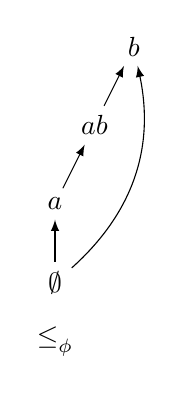
\begin{tikzpicture}
		\node at (0,-0.75){$\le^{\exh}_{\phi}$};
		\node at (0,0)(e){$\emptyset$};
		\node at (0,1)(a){$a$};
		\node at (0.5,2)(ab){$ab$};
		\node at (1,3)(b){$b$};
		\path[-latex]
			(e)edge(a)
			(e)edge[bend right=30](b)
			(a)edge(ab)
			(ab)edge(b);
	\end{tikzpicture}
	\caption{
		The exhaustive $\re$-revealed $\L_{\horn}$-assignment 
		is not guaranteed to be transitive.
	}
	\label{fig:6-hhh-revision-exhaustive-revealed-not-transitive}
\end{figure}

\begin{xmpl}{$\le^{\exh}_{\phi}$ might not be transitive}{6-hhh-revision-exhaustive-revealed-not-transitive}
	Consider an $\HHH$-revision operator $\re$ such that,
	for the set of atoms $\Atoms=\{a,b\}$,
	delivers the following results:
	$[\phi\re\px_{a,ab}]=\{a\}$,
	$[\phi\re\px_{ab,b}]=\{ab\}$
	and
	$[\phi\re\px_{a,b}]=\{\emptyset\}$.
	From this we infer that 
	$a<^{\exh}_{\phi} ab$,
	$ab <^{\exh}_{\phi} b$, 
	$\emptyset <^{\exh}_{\phi} a$
	and 
	$\emptyset <^{\exh}_{\phi} b$.
	These comparisons are depicted in 
	Figure \ref{fig:6-hhh-revision-exhaustive-revealed-not-transitive}.
	In propositional logic we would be able to use 
	postulates $\ppr{5-6}$ to infer from
	the result for $\phi\re\px_{a,ab}$ and for
	$\phi\re\px_{ab,b}$
	that a choice over interpretations $a$, $ab$ and $b$
	has to select $a$;
	based on this, we would infer that the choice over $a$ and $b$
	has to select $a$ as well, meaning that $a$ is considered better 
	than $b$.
	However, in the Horn fragment there is no way of 
	enforcing choice over $a$, $ab$ and $b$,
	since $\{a,b,ab\}$ is not $\horn$-closed.
	This makes it possible for the result to be $\emptyset$
	when revising by $\px_{a,b}$,
	leaving $a$ and $b$ incomparable in $\le^{\exh}_{\phi}$.
\end{xmpl}

Example \ref{ex:6-hhh-revision-exhaustive-revealed-not-transitive}
illustrates one of the consequences of restricting the
language: since there are certain configurations 
of outcomes the agent never gets to see,
the revision operator
becomes less precise at identifying the relationship 
between certain outcomes:
if $w_1\subseteq w_2$ or $w_2 \subseteq w_1$, 
then $\{w_1,w_2\}$ is $\horn$-closed and $\phi\re\px_{1,2}$
behaves as in propositional logic;
but if $w_1$ and $w_2$ are subset-incomparable,
then there is no way to make a comparison only between the two of them,
and the revealed relation may feature patches where
the revision operators has nothing informative to say.

Nevertheless, a glance at
Example \ref{ex:6-hhh-revision-exhaustive-revealed-not-transitive}
suggests an easy fix:
note that the transitive closure of $\le^{\exh}_{\phi}$,
as depicted in Figure \ref{fig:6-hhh-revision-exhaustive-revealed-not-transitive},
is an ordering extension of $\le^{\exh}_{\phi}$, as defined in Section \ref{sec:2-choice-functions},
i.e., a relation that preserves all the comparisons
in $\le^{\exh}_{\phi}$, including the strict ones.
Thus, even if the revision operator does not explicitly state
that $a$ is better than $b$, given the prior information $\phi$,
we may still attempt to infer this from the intermediary comparisons 
of $a<^{\exh}_{\phi} ab$ and $ab <^{\exh}_{\phi} b$.
Importantly, adding the comparison $a <^{\exh}_{\phi} b$
to $\le^{\exh}_{\phi}$ does not misrepresent $\re$: 
the augmented relation underlies the same revision operator.
This raises the hope of a general strategy,
and we will soon see the conditions under which this strategy is successful.

So far, so good.
The problem, as has been already documented \cite{DelgrandeP15,DelgrandePW18},
is that these elements alone are not enough to 
deliver a representation result. 
A first indication that more needs to be done is the fact that
assignments based on standard, distance-based preorders 
(either total or partial, r-faithful or not) 
cannot be used to induce $\HHH$-revision operators.

\begin{figure}\centering
	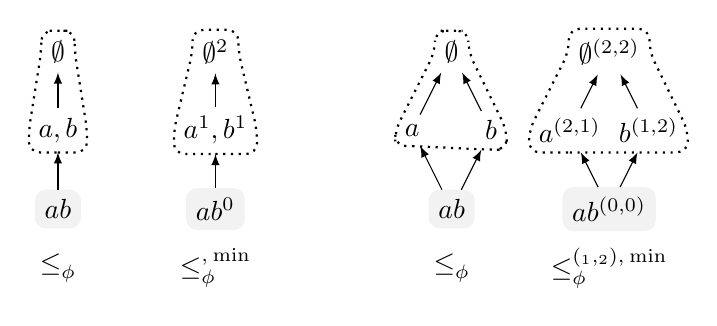
\begin{tikzpicture}
		\node at (0,-0.75){$\le^{\totalPre}_{\phi}$};
		\node at (0,0)(ab){$ab$};
		\node at (0,1)(a){$a,b$};
		\node at (0,2)(e){$\emptyset$};
		\path[-latex]
			(ab) edge (a)
			(a) edge (e);
		\fill[opacity=0.05,rounded corners=4]
			(ab.south)--
			(ab.south west)--
			(ab.west)--
			(ab.north west)--
			(ab.north)--
			(ab.north east)--
			(ab.east)--
			(ab.south east)--
			(ab.south);
		\draw[thick,dotted, rounded corners=4]
			(a.south)--
			(a.south east)--
			(a.east)--
			(e.east)--
			(e.north east)--
			(e.north)--
			(e.north west)--
			(e.west)--
			(a.west)--
			(a.south west)--
			(a.south);


		\node at (2,-0.75){$\le^{\hamming,\:\min}_{\phi}$};
		\node at (2,0)(ab){$ab^{0}$};
		\node at (2,1)(a){$a^{1},b^{1}$};
		\node at (2,2)(e){$\emptyset^{2}$};
		\path[-latex]
			(ab) edge (a)
			(a) edge (e);
		\fill[opacity=0.05,rounded corners=4]
			(ab.south)--
			(ab.south west)--
			(ab.west)--
			(ab.north west)--
			(ab.north)--
			(ab.north east)--
			(ab.east)--
			(ab.south east)--
			(ab.south);
		\draw[thick,dotted, rounded corners=4]
			(a.south)--
			(a.south east)--
			(a.east)--
			(e.east)--
			(e.north east)--
			(e.north)--
			(e.north west)--
			(e.west)--
			(a.west)--
			(a.south west)--
			(a.south);

		\node at (5,-0.75){$\le^{\partialPre}_{\phi}$};
		\node at (5,0)(ab){$ab$};
		\node at (4.5,1)(a){$a$};
		\node at (5.5,1)(b){$b$};
		\node at (5,2)(e){$\emptyset$};
		\path[-latex]
			(ab) edge (a)
			(a) edge (e)
			(ab) edge (b)
			(b) edge (e);
		\fill[opacity=0.05,rounded corners=4]
			(ab.south)--
			(ab.south west)--
			(ab.west)--
			(ab.north west)--
			(ab.north)--
			(ab.north east)--
			(ab.east)--
			(ab.south east)--
			(ab.south);
		\draw[thick,dotted, rounded corners=4]
			(a.south)--
			(b.south)--
			(b.south east)--
			(b.east)--
			(e.east)--
			(e.north east)--
			(e.north)--
			(e.north west)--
			(e.west)--
			(a.west)--
			(a.south west)--
			(a.south);	

		\node at (7,-0.75){$\le^{(\dd_{1},\dd_{2}),\:\min}_{\phi}$};
		\node at (7,0)(ab){$ab^{(0,0)}$};
		\node at (6.5,1)(a){$a^{(2,1)}$};
		\node at (7.5,1)(b){$b^{(1,2)}$};
		\node at (7,2)(e){$\emptyset^{(2,2)}$};
		\path[-latex]
			(ab) edge (a)
			(a) edge (e)
			(ab) edge (b)
			(b) edge (e);
		\fill[opacity=0.05,rounded corners=4]
			(ab.south)--
			(ab.south west)--
			(ab.west)--
			(ab.north west)--
			(ab.north)--
			(ab.north east)--
			(ab.east)--
			(ab.south east)--
			(ab.south);
		\draw[thick,dotted, rounded corners=4]
			(a.south)--
			(b.south)--
			(b.south east)--
			(b.east)--
			(e.east)--
			(e.north east)--
			(e.north)--
			(e.north west)--
			(e.west)--
			(a.west)--
			(a.south west)--
			(a.south);	
	\end{tikzpicture}
	\caption{
		Preorders $\le^{\totalPre}_{\phi}$ and $\le^{\partialPre}_{\phi}$
		for $\phi=a\land b\land\lnot c$ and $\mu=\lnot(a\land b)\land \lnot c$.
		Models of $\phi$ are shaded in gray, 
		models of $\mu$ are surrounded by the 
		dotted line.
		Neither of the preorders
		$\le^{\totalPre}_{\phi}$ and $\le^{\partialPre}_{\phi}$
		delivers a $\horn$-closed set of interpretations,
		and thus cannot be used to model 
		$\HHH$-revision operators.
		These preorders coincide with $\le^{\hamming,\:\min}_{\phi}$
		and $\le^{(\dd_{1},\dd_{2}),\:\min}_{\phi}$,
		as presented in Example \ref{ex:3-revision-dmin}.
	}
	\label{fig:6-hhh-revision-standard-ops-no-good}
\end{figure}

\begin{xmpl}{Preorders that do not induce an $\HHH$-revision operator}{6-hhh-revision-standard-ops-no-good}
	For the set of atoms $\Atoms=\{a,b,c\}$,
	consider formulas $\phi=a\land b\land\lnot c$
	and $\mu=\lnot (a\land b)\land\lnot c$.
	We have that $[\phi]=\{ab\}$ and
	$[\mu]=\{\emptyset,a,b\}$.
	Both $\phi$ and $\mu$ are Horn formulas,
	and are thus valid inputs to an $\HHH$-revision operator.
	Consider, however, a total assignment $\as^{\totalPre}$
	and a partial assignment $\as^{\partialPre}$
	that assigns to $\phi$ 
	the preorders
	$\le^{\totalPre}_{\phi}$ and  $\le^{\partialPre}_{\phi}$,
	respectively,
	both depicted in Figure \ref{fig:6-hhh-revision-standard-ops-no-good}.
	We obtain that:
	\begin{align*}
		\min_{\le^{\totalPre}_{\phi}}[\mu] &=\min_{\le^{\partialPre}_{\phi}}[\mu]\\
											&= \{a,b\},	
	\end{align*}
	and hence $[\phi\re^{\totalPre}\mu]=[\phi\re^{\partialPre}\mu]=\{a,b\}$.
	Since $\cl_{\horn}(\{a,b\})=\{\emptyset,a,b\}\neq\{a,b\}$,
	it follows that 
	$[\phi\re^{\totalPre}\mu]$ and $[\phi\re^{\partialPre}\mu]$ 
	cannot be represented as a Horn formula,
	i.e., the $\as^{\totalPre}$-induced and $\as^{\partialPre}$-induced
	revision operators do not work as 
	$\HHH$-revision operators.

	This finding is significant,
	because $\le^{\totalPre}_{\phi}$
	coincides on the models of $\phi$ and $\mu$ 
	with the preorder generated 
	by many of the distance-based
	assignments we looked at in Section \ref{sec:3-revision}
	(the set of atoms is considered to coincide with $\Atoms$ in that example),
	namely with 
	$\le^{\hamming,\:\min}_{\phi}$,
	$\le^{\hamming,\:\leximin}_{\phi}$,
	$\le^{\hamming,\:\max}_{\phi}$,
	$\le^{\hamming,\:\leximax}_{\phi}$
	and
	$\le^{\hamming,\:\ssum}_{\phi}$.
	Also, $\le^{\partialPre}_{\phi}$
	coincides on the models of $\phi$ and $\mu$
	with the partial preorder $\le^{(\dd_{1},\dd_{2}),\:\min}_{\phi}$
	presented in Example \ref{ex:3-revision-dmin}.
\end{xmpl}

Example \ref{ex:6-hhh-revision-standard-ops-no-good}
shows that, like in Section \ref{sec:6-revision-hph},
there are certain preorders bound to deliver results 
that cannot be recast as Horn formulas.
Unfortunately, these preorders appear in
the distance-based assignments we have introduced
in Section \ref{sec:3-revision} for $\L$-revision operators.
The upshot, then, is that none of these assignments
can be repurposed for $\HHH$-revision.

The problem highlighted by Example \ref{ex:6-hhh-revision-standard-ops-no-good}
is that properties $\oor{1-7}$, by themselves,
make an $\L_{\horn}$-assignment $\as$ on interpretations
ill-equipped to induce a well-defined $\HHH$-revision operator.
The solution, as for $\HPH$-revision operators, 
is to rein in the preorders we are looking at.
The purpose, here, is to find a restriction on 
$\L_{\horn}$-assignments that ensures 
they deliver $\horn$-closed results when the new information is 
a Horn formula.
This is done via the following property, intended to hold for 
any Horn formula $\phi$ and interpretations $w_1$ and $w_2$:

\begin{description}
	\item[($\oor{\HC}$)] For any Horn formula $\mu$, 
		it holds that $\min_{\le_{\phi}}[\mu]$ if $\horn$-closed.
\end{description}

% We will do this in two ways, depending on whether the preorders 
% we are working with are total or partial.

% Total preorders, we know from Section \ref{sec:3-revision},
% go hand in hand with postulates $\ppr{1-6}$, but we are 
% beginning to see that for the Horn fragment these elements 
% may not be enough.

% \begin{description}
% 	\item[($\oor{\TCMPL}$)] 
% 		If $w_1 \approx_{\phi}w_2$, 
% 		then $(w_1\cap w_2) \le_{\phi} w_1$ or $(w_1\cap w_2) \le_{\phi} w_2$.	
% 		% If $w_1 \not<_{\phi}w_2$ and $w_2\not<_{\phi}w_1$, 
% 		% then $(w_1\cap w_2) \in\min_{\le_{\phi}}\cl_{\horn}(\{w_1,w_2\})$.
% \end{description}

\begin{figure}\centering
	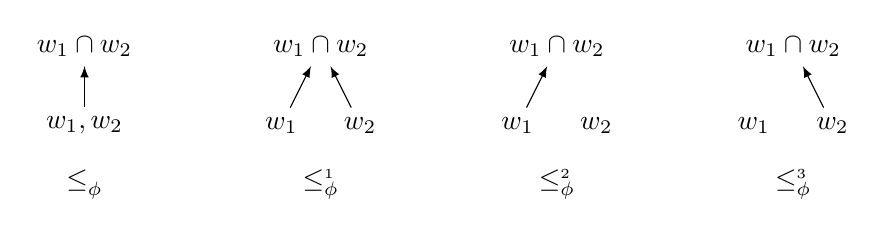
\begin{tikzpicture}
		\node at (0,-0.75)(1){$\le^{\totalPre}_{\phi}$};
		\node at (0,0)(1){$w_1,w_2$};
		\node at (0,1)(2){$w_1\cap w_2$};
		\path[-latex] (1)edge(2);

		\node at (3,-0.75){$\le^{\partialPre_1}_{\phi}$};
		\node at (2.5,0)(1){$w_1$};
		\node at (3.5,0)(2){$w_2$};
		\node at (3,1)(3){$w_1\cap w_2$};
		\path[-latex] (1)edge(3)(2)edge(3);

		\node at (6,-0.75){$\le^{\partialPre_2}_{\phi}$};
		\node at (5.5,0)(1){$w_1$};
		\node at (6.5,0)(2){$w_2$};
		\node at (6,1)(3){$w_1\cap w_2$};
		\path[-latex] (1)edge(3);

		\node at (9,-0.75){$\le^{\partialPre_3}_{\phi}$};
		\node at (8.5,0)(1){$w_1$};
		\node at (9.5,0)(2){$w_2$};
		\node at (9,1)(3){$w_1\cap w_2$};
		\path[-latex] (2)edge(3);
	\end{tikzpicture}	
	\caption{
		Preorders, total and partial, that deliver results that 
		are not $\horn$-closed when revising by a Horn formula $\mu$, 
		with $[\mu]=\{w_1,w_2,w_1\cap w_2\}$.
		It is assumed that $w_1\nsubseteq w_2$ and $w_2\nsubseteq w_1$,
		such that $w_1\cap w_2$ is an interpretation distinct from both $w_1$ and $w_2$.
		The goal of property $\oor{\HC}$ is to prevent the occurrence of these configurations.
	}
	\label{fig:6-hhh-revision-non-compliant-preorders}
\end{figure}

Property $\oor{\HC}$, where `$\HC$' 
stands for \emph{Horn compliance} \cite{DelgrandeP15,DelgrandePW18},
guarantees that the $\le_{\phi}$-minimal elements of $[\mu]$,
when $\mu$ is a Horn formula, can be represented by a Horn formula.
Property $\oom{\HC}$ works for both total and partial preorders,
and its role, essentially, is to rule out situations such as the ones 
in Figure \ref{fig:6-hhh-revision-non-compliant-preorders},
where revision by a Horn formula yields a set of interpretations 
that cannot be expressed as a Horn formula.
% In deference to this fact,
An $\L_{\horn}$-assignment $\as$ on interpretations 
is \emph{Horn compliant} if it satisfies property $\oor{\HC}$.
It is straightforward to see that
property $\oor{\HC}$ is a condition that is both necessary and sufficient
for a propositional revision operator to function as an $\HHH$-revision operator.


% Property $\oor{\TCMPL}$, where `$\TCMPL$' denotes \emph{triples compliance},
% says that if interpretations $w_1$ and $w_2$ are equally good in $\le_{\phi}$,
% then $w_1\cap w_2$ should also be considered as least as good as $w_1$ and $w_2$.
% If $w_1 \subseteq w_2$ or $w_2 \subseteq w_1$, then property $\oor{\TCMPL}$
% is trivially satisfied, but if $w_1$ and $w_2$ are subset-incomparable,
% then property $\oor{\TCMPL}$ is more meaningful and its role, essentially,
% is to eliminate the configuration in Figure \ref{fig:6-hhh-revision-non-compliant-preorders}.
% The intuition behind this requirement is that if
% $w_1$ and $w_2$ are subset-incomparable,
% then the choice over $\{w_1,w_2,w_1\cap w_2\}$
% cannot consist of $w_1$ and $w_2$ alone,
% since this can yield a revision result that is not $\horn$-closed.
% Thus, property $\oor{\TCMPL}$ forces that the
% choice over interpretations $\{w_1,w_2,w_1\cap w_2\}$
% contains the interpretation $w_1\cap w_2$ as well,
% guaranteeing a $\horn$-closed result.
% The guiding intuition is that if 
% The solution, then, is to ensure that the preorder $\le_{\phi}$ is never 
% in a situation where $w_1$ and $w_2$ can occur as the minimal elements in 
% $\cl_{\horn}(\{w_1,w_2\})$.

% Property $\oor{\TCMPL}$ looks convoluted because it packs just as much information 
% as needed to work for both partial and total preorders.
% We can unpack it into a more understandable format
% if we look at the configurations it is indended to prevent.
% If $\le_{\phi}$ is assumed to be a total preorder, then the precondition 
% in property $\oor{\TCMPL}$ becomes equivalent to saying that $w_1\approx_{\phi} w_2$
% and $\oor{\TCMPL}$, as a whole, boils down to the following property, 
% holding for any Horn formula $\phi$ and interpretations $w_1$ and $w_2$:

% \begin{description}
% 	\item[($\oor{\TCMPL_\totalPre}$)] If $w_1 \approx_{\phi}w_2$, 
% 		then $(w_1\cap w_2) \le_{\phi} w_1$ or $(w_1\cap w_2) \le_{\phi} w_2$.
% \end{description}



% In other words, property $\oor{\TCMPL_\totalPre}$ eliminates the 
% configuration depicted by $\le^{\totalPre}_{\phi}$ 
% in Figure \ref{fig:6-hhh-revision-non-compliant-preorders},
% in which $\min_{\le^{\totalPre}_{\phi}}\{w_1,w_2,w_1\cap w_2\}=\{w_1,w_2\}$.
% Note that $\{w_1,w_2\}$ is not $\horn$-closed,
% and is therefore not a viable result for an $\HHH$-revision operator.

% If $\le_{\phi}$ is assumed to be partial, then property $\oor{\TCMPL}$
% eliminates the configurations depicted by 
% $\le^{\partialPre_1}_{\phi}$,
% $\le^{\partialPre_2}_{\phi}$
% and
% $\le^{\partialPre_3}_{\phi}$
% in Figure \ref{fig:6-hhh-revision-non-compliant-preorders}.
% In all three of these cases it holds that 
% $\min_{\le^{\partialPre_i}_{\phi}}\{w_1,w_2,w_1\cap w_2\}=\{w_1,w_2\}$,
% for $i\in\{1,2,3\}$,
% and it is in our interest to prevent such configurations from occurring.
% Note that the problematic cases all involve pairs of interpretations 
% $w_1$ and $w_2$ that are subset-incomparable, 
% and cannot therefore be represented precisely by a Horn formula. 
% If $w_1 \subseteq w_2$ or $w_2 \subseteq w_1$, then property $\oor{\TCMPL}$ is trivially true.

% Property $\oor{\TCMPL}$ is formulated for pairs $\{w_1,w_2\}$ of interpretations
% and makes sure that a choice 

% However, our intention is to cover any $\horn$-closed 
% set $\W$ of interpretations, in order to ensure that its $\le_{\phi}$-minimal 
% elements can represent a Horn formula: 
% the idea here is that we want to foolproof $\le_{\phi}$ such that, 
% whatever the new information $\mu$ is, 
% the result $\min_{\le_\phi}[\mu]$ of revision 
% by $\mu$ can be recast as a Horn formula.
% If $\le_{\phi}$ is a total preorder, 
% property $\oor{\TCMPL}$ allows us to do that.

% \begin{prp}{}{6-hhh-revision-triples-horn-compliance}
% 	If $\le_{\phi}$ is a total preorder, then 
% 	$\le_{\phi}$ satisfies property $\oor{\TCMPL}$
% 	if and only if, 
% 	for any Horn formula $\mu$,
% 	it holds that $\min_{\le_{\phi}}[\mu]$ is $\horn$-closed.
% \end{prp}
% \begin{prf*}{}{}%
% 	(``$\Rightarrow$'')
% 	Suppose $\le_{\phi}$ satisfies property $\oor{\TCMPL}$
% 	and $min_{\le_{\phi}}[\mu]$ is not $\horn$-closed.
% 	Then there exist interpretations 
% 	$w_1$ and $w_2$ in $\min_{\le_{\phi}}[\mu]$ such that 
% 	$w_1\cap w_2\notin\min_{\le_{\phi}}[\mu]$.
% 	Since $\le_{\phi}$ is total, this implies that $w_1\approx_{\phi}w_2<_{\phi}w_1\cap w_2$,
% 	which contradicts property $\oor{\TCMPL}$.

% 	(``$\Leftarrow$'')
% 	Take two interpretations $w_1$ and $w_2$ such that $w_1\approx_{\phi}w_2$,
% 	and an $\L_{\horn}$-proxy $\px_{1,2}$ of $\{w_1,w_2\}$.
% 	We obtain that $\min_{\le_{\phi}}\px_{1,2}$ is $\horn$-closed,
% 	which implies that $w_1\cap w_2\in \min_{\le_{\phi}}\px_{1,2}$,
% 	i.e., $w_1\cap w_1\le_{\phi}w_1$.
% \end{prf*}


% \begin{thm}{}{6-hhh-revision-equiv-TCMPL}
% 	If $\re$ is an $\L$-revision operator
% 	and $\as$ is an $\L$-assignment on interpretations
% 	that represents it,
% 	then $\re$ is an $\HHH$-revision operator, 
% 	when restricted to Horn formulas,
% 	if and only if $\as$ satisfies property $\oor{\TCMPL}$,
% 	when restricted to Horn formulas.
% \end{thm}
% \begin{prf*}{}{}%
% 	We have that $\re$ being an $\HHH$-revision operator
% 	is equivalent to 
% 	$\min_{\le_{\phi}}[\mu]$ being $\horn$-closed,
% 	for any Horn formulas $\phi$ and $\mu$,
% 	which, using Proposition \ref{prop:6-hhh-revision-triples-horn-compliance},
% 	is equivalent to property $\oor{\TCMPL}$ being satisfied.
% \end{prf*}


% Horn compliance, however, :
% it guarantees that the result of an 
% $\as$-induced revision operator can be expressed 
% as a Horn formula,
% and that only such assignments can represent 
% $\HHH$-revision operators,
% but it does not ensure 
% that such formulas have other 
% desirable properties.
% We will see that these properties can be 
% guaranteed by adding on properties $\oor{1-7}$.

With the expressibility issue fixed, the next step is to 
look at the effect of postulates $\ppr{1-6}$, or $\ppr{1-5}$ and $\ppr{7-8}$,
and connect them to properties $\oor{1-7}$.
However, another problem rears its head:
it turns out that restricted to Horn formulas, 
the revision postulates 
end up saying less than their propositional counterparts,
to the point where they can now induce
unwanted assignments. 
To understand this issue, it is best to 
look at total and partial preorders separately.

\subsubsection{Total preorders}
Total preorders, we know from Section \ref{sec:3-revision},
go hand in hand with postulates $\ppr{1-6}$, but we are 
beginning to see that for the Horn fragment these elements 
may not be enough.
As has been observed, one outstanding problem is the 
presence of non-transitive cycles in assignments 
that can represents $\HHH$-revision operators
that satisfy postulates $\ppr{1-6}$.

\begin{figure}\centering
	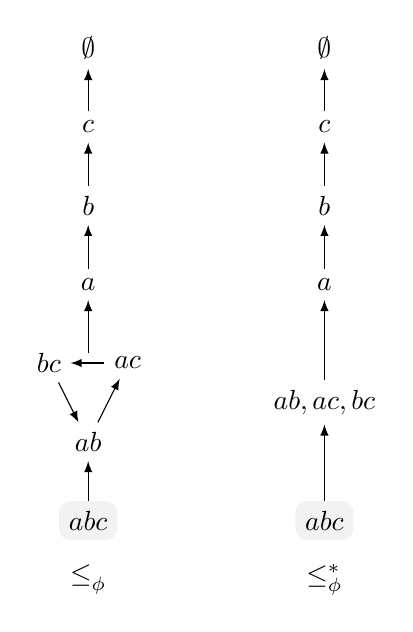
\begin{tikzpicture}
		\node at (0,-0.75){$\le^{\exh}_{\phi}$};
		\node at (0,0)(abc){$abc$};
		\node at (0,1)(ab){$ab$};
		\node at (0.5,2)(ac){$ac$};
		\node at (-0.5,2)(bc){$bc$};
		\node at (0,2)(anchor1){};
		\node at (0,3)(a){$a$};
		\node at (0,4)(b){$b$};
		\node at (0,5)(c){$c$};
		\node at (0,6)(e){$\emptyset$};
		\path[-latex]
		(abc) edge (ab)
		(ab) edge (ac)
		(ac) edge (bc)
		(bc) edge (ab)
		(anchor1) edge (a)
		(a) edge (b)
		(b)edge(c)
		(c)edge(e);		
	\fill[opacity=0.05,rounded corners=4]
		(abc.south)--
		(abc.south west)--
		(abc.west)--
		(abc.north west)--
		(abc.north)--
		(abc.north east)--
		(abc.east)--
		(abc.south east)--
		(abc.south);

	\node at (3,-0.75){$\le^{\ast}_{\phi}$};
	\node at (3,0)(abc){$abc$};
	\node at (3,1.5)(ab){$ab,ac,bc$};
	\node at (3,3)(a){$a$};
	\node at (3,4)(b){$b$};
	\node at (3,5)(c){$c$};
	\node at (3,6)(e){$\emptyset$};
	\path[-latex]
		(abc) edge (ab)
		(ab) edge (a)
		(a) edge (b)
		(b)edge(c)
		(c)edge(e);		
	\fill[opacity=0.05,rounded corners=4]
		(abc.south)--
		(abc.south west)--
		(abc.west)--
		(abc.north west)--
		(abc.north)--
		(abc.north east)--
		(abc.east)--
		(abc.south east)--
		(abc.south);
	\end{tikzpicture}
	\caption{
		The exhaustive revealed ranking $\le^{\exh}_{\phi}$
		for an $\HHH$-revision operator $\re$ that satisfies
		postulates $\ppr{1-5}$ and $\ppr{7-8}$
		and $\phi=a\land b\land c$,
		together with the ranking $\le^{\ast}_{\phi}$
		obtained as the transitive closure of $\le^{\exh}_{\phi}$.
		The ranking $\le^{\exh}_{\phi}$
		contains a non-transitive 
		cycle between $ab$, $ac$ and $bc$,
		and behaves like a total preorder otherwise.
		The non-transitive cycle goes undetected 
		when $\re$ processes 
		only Horn formulas.
		The transitive closure $\le^{\ast}_{\phi}$
		of $\le^{\exh}_{\phi}$
		fixes the non-transitivity issue but
		does not represent the revision operator $\re$
		anymore.
		}
	\label{fig:6-hhh-revision-cycle}
\end{figure}

\begin{xmpl}{\cite{DelgrandeP15,DelgrandePW18}}{6-hhh-revision-cycles}
	For the set of atoms $\Atoms=\{a,b,c\}$
	and the formula $\phi=a\land b\land c$,	
	consider an $\HHH$-revision operator $\re$
	that induces the exhaustive revealed plausibility
	relation $\le^{\exh}_{\phi}$ in Figure \ref{fig:6-hhh-revision-cycle}.
	In other words, it holds that 
	$[\phi\re\px_{ab,ac}]=\{ab\}$,
	$[\phi\re\px_{ac,bc}]=\{ac\}$,
	$[\phi\re\px_{bc,ab}]=\{bc\}$,
	and so on:
	the results of the revision operator on
	all the possible inputs can be read off 
	from Figure \ref{fig:6-hhh-revision-cycle}.

	The significant detail about the 
	revealed relation $\le^{\exh}_{\phi}$
	is that it 
	behaves like a total preorder everywhere 
	except on $ab$, $ac$ and $bc$,
	which are fixed into a non-transitive cycle.
	In other words, $\re$ decides
	that $ab <^{\exh}_{\phi} ac <^{\exh}_{\phi} bc <^{\exh}_{\phi} ab$,
	which implies that $\le_{\phi}$ does not satisfy property $\oor{3}$
	on $ab$, $ac$ and $bc$.

	We would expect that the failure of $\le^{\exh}_{\phi}$ to 
	satisfy property $\oor{3}$
	translates into $\re$ 
	not satisfying some of the revision postulates:
	and if we were working in propositional logic,
	this would indeed be the result.
	In propositional logic we can always revise by a 
	propositional formula
	that has exactly $ab$, $ac$ and $bc$ as its models;
	revision with this formula 
	together with postulate $\ppr{3}$ 
	implies that $\min_{\le^{\exh}_{\phi}}\{ab,ac,bc\}$
	has to be non-empty,
	contrary to the present situation:
	in the framework of propositional logic 
	the regular postulates $\ppr{1-6}$ make 
	a revision operator such as the operator $\re$ specified here 
	impossible.

	Interestingly, in the Horn fragment the operator $\re$
	turns out to be a perfectly legal $\HHH$-revision operator:
	it can be checked that $\re$ satisfies postulates $\ppr{1-6}$
	\cite{DelgrandeP15,DelgrandePW18}.
	The reason why the cycle manages to slip through undetected
	is that in the Horn fragment there is no formula
	that has exactly $ab$, $ac$ and $bc$ as its models,
	since $\{ab,ac,bc\}$ is not $\horn$-closed.
	The closest we can come to this is by 
	using an $\L_{\horn}$-proxy 
	$\px_{ab,ac,bc}$ of $\{ab,ac,bc\}$,
	but $[\px_{ab,ac,bc}]=\cl_{\horn}(\{ab,ac,bc\})=\{\emptyset,a,b,c,ab,ac,bc\}$,
	and simply asking 
	that $\min_{\le^{\exh}_{\phi}}[\px_{ab,ac,bc}]$ is non-empty 
	does not prevent the cycle.
	
	A tentative fix for this situation is to 
	replace $\le^{\exh}_{\phi}$,
	as in Example \ref{ex:6-hhh-revision-exhaustive-revealed-not-transitive}	
	with its transitive closure $\le^{\ast}_{\phi}$,
	also depicted in Figure \ref{fig:6-hhh-revision-cycle}.
	This has the effect of flattening the cycle
	by introducing indifference between $ab$, $bc$ and $ac$.
	The downside of this move however, is that $\le^{\ast}_{\phi}$
	does not preserve the information provided by $\re$:
	we can see this by looking at the revision operator $\re^{\ast}$ induced 
	by the preorder $\le^{\ast}_{\phi}$, 
	and comparing it to $\re$: 
	we have that
	$[\phi\re\px_{ab,ac}]=\{ab\}$,
	i.e.,
	$\min_{\le^{\exh}_{\phi}}\{ab,ac,a\} = \{ab\}$,
	whereas 
	$\min_{\le^{\ast}_{\phi}}\{ab,ac,a\} = \{ab,ac\}$,
	i.e., 
	$[\phi\re^{\ast}\px_{ab,ac}]=\{ab,ac\}$.
	The cycle-free transitive closure of $\le^{\exh}_{\phi}$
	represents a different revision operator, 
	one that does not even return a Horn formula!

	The moral here is that 
	the preorder $\le^{\exh}_{\phi}$
	depicted in Figure \ref{fig:6-hhh-revision-cycle}
	cannot be extended to a total preorder while
	still remaining faithful to the revision operator $\re$:
	eliminating the cycle between $ab$, $bc$ and $ac$
	would lead to $\le^{\exh}_{\phi}$ misrepresenting $\re$.
	% Note that the cycle is obtained even if we use the 
	% exclusive $\re$-revealed assignment instead of the
	% exhaustive one.
	The cycle, here, is unavoidable.
\end{xmpl}

In Example \ref{ex:6-hhh-revision-exhaustive-revealed-not-transitive}
we encountered an exhaustive $\HHH$-revision operator 
that induced a non-transitive ranking on outcomes,
but this ranking could be made transitive by 
filling in the gaps with the
comparisons inferred by transitivity.
Example \ref{fig:6-hhh-revision-cycle}
shows that there are exhaustive $\HHH$-revision operators 
inducing rankings that are not only non-transitive,
but that cannot even be made transitive:
postulates $\ppr{1-6}$,
the most demanding revision postulates we have,
not only fail to notice the cycle between $ab$, $ac$ and $bc$,
but allow the agent to revise in a way that makes the cycle
compulsory.
This is a direct result of the Horn fragment's inability
to capture certain sets of interpretations:
whereas in propositional logic we would be able 
to leverage postulates $\ppr{1-6}$
to make sure that the revealed exhaustive ranking is transitive,
in the Horn fragment this move is not possible.

% Example \ref{fig:6-hhh-revision-cycle} 
% throws a wrench in the works:
% $\HHH$-revision operators exist for which this is not possible,
% i.e., that cannot be rationalized by transitive plausibility relations.
% In propositional logic 
% such operators are disallowed by postulates $\ppr{1-6}$,
% but in the Horn fragment the same postulates fail 
% to provide the same guarantees.

% Does this mean that there is no guarantee that 
% revision for Horn formulas can be rationalized in a 
% meaningful way?

One way to deal with this situation is to make sure that 
an exhaustive $\HHH$-revision operator does not 
revise in a way that paints it into a non-transitive corner,
and it is here that the literature on rational choice proves useful,
as it suggests a tool of proven efficacy: Suzumura consistency.
Recall Theorem \ref{thm:2-suzumura-consistency},
saying that Suzumura consistency 
is both a necessary and sufficient condition for a binary relation to
have an extension that is a total preorder.
In the context of revision, we can formulate Suzumura consistency
as a property that applies to preorders in an assignment $\as$ on interpretations.
Thus, for any 
Horn formula $\phi$
and interpretations $w_1$, \dots, $w_n$, 
the property is as follows:

\begin{description}
	\item[($\oor{\SCON}$)] If $w_1 \le_{\phi}\dots \le_{\phi}w_n$,
		then $w_{n}\not<_{\phi} w_{1}$.
\end{description}

Property $\oor{\SCON}$, 
with $\SCON$ standing for \emph{Suzumura consistency},
has a natural reading: 
if $w_1$ is at least as good as $w_2$ according to $\le_\phi$,
$w_2$ is at least as good as $w_3$,
and so on, all the way to $w_n$, then
the betterness of $w_1$ should propagate down the line,
i.e., the last outcome in this sequence cannot 
be strictly better than $w_1$.
Property $\oor{\SCON}$ is, of course, implied by transitivity,
i.e., by property $\oor{3}$,
but if property $\oor{3}$ cannot be enforced then $\oor{\SCON}$
is the safest bet, as long as $\oor{\SCON}$ itself can be enforced.

How can we make sure that $\HHH$-revision operators 
describe only Suzumura consistent preorders? 
By supplementing the standard set of postulates
with a special postulate, tailored specifically for property $\oor{\SCON}$.
% Before going ahead with this strategy, a few observations are required.
% First, the additional postulate is meant to ensure that the assignment inferred 
% from the revision operator $\re$, and intended to 
% represent $\re$, satisfies property $\oor{\SCON}$:
% it turns out, however, that it matters how the assignment is inferred,
% i.e., whether it is the exhaustive or exclusive. 
% Since the exhaustive assignment is used when the base set postulates is $\ppr{1-6}$
% and the exclusive assignment is used for postulates $\ppr{1-5}$ and $\ppr{7-8}$,
% we will need two postulates, one for each case.
We will formulate the postulate using 
the notion of an $\L_{\horn}$-proxy
of a set $\W$ of interpretations, 
introduced in Section \ref{sec:6-horn-fragment}: 
recall, this is a Horn formula $\px_{\W}$
such that $[\px_{\W}]=\cl_{\horn}(\W)$.
We will apply this notion to singletons $\{w_i\}$ 
and pairs $\{w_i,w_j\}$ of interpretations,
in which case we write $\px_{i}$ and $\px_{i,j}$
instead of $\px_{w_i}$ and $\px_{w_i,w_j}$, respectively.
Since singleton sets of interpretations are $\horn$-closed,
it holds that $[\px_{i}]=\cl_{\horn}(\{w_i\})=\{w_i\}$.
Pairs of interpretations are not necessarily $\horn$-closed,
in which case $[\px_{i,j}]$ may contain
the additional interpretation $w_i\cap w_j$.

The additional postulate, or, more precisely, 
postulate schema, is intended 
to work for the exhaustive revealed assignment,
and meant to apply for any Horn formula $\phi$, integer $n$,
interpretations $w_1$, \dots, $w_n$
and their associate $\L_{\horn}$-proxy formulas:

\begin{description}
	\item[($\ppr{\SCON}$)]
		If 
			$(\phi\re\px_{1,2})\land\px_{1}$ is consistent,
			\dots,
			$(\phi\re\px_{n-1,n})\land\px_{n-1}$ is consistent,
		then it does not hold that both
		$(\phi\re\px_{n,1})\land\px_{n}$ is consistent
		and that $(\phi\re\px_{n,1})\land\px_{1}$ is inconsistent.
\end{description}

Postulate $\ppr{\SCON}$ expresses the same idea as property $\oor{\SCON}$,
but using formulas and the revision operator 
instead of interpretations and the preorder.
Note that this connection applies only if the preorder
is part of the exhaustive $\re$-revealed assignment.

\begin{thm}{}{6-SCON-scon}
	If $\re$ is an $\HHH$-revision operator 
	and $\as^{\exh}$ is the $\re$-revealed exhaustive assignment, then
	$\re$ satisfies postulate $\ppr{\SCON}$
	if and only if 
	$\as^{\exh}$ satisfies property $\oor{\SCON}$.
\end{thm}
\begin{prf*}{}{}%
	(``$\Rightarrow$'')
	Assume $\re$ satisfies postulate $\ppr{\SCON}$ and 
	take interpretations $w_1$, \dots, $w_n$
	such that $w_1 \le^{\exh}_{\phi}\dots \le^{\exh}_{\phi} w_n$,
	and suppose $w_n<^{\exh}_{\phi}w_1$.
	It follows, first, that $w_1\in[(\phi\re\px_{1,2})\land\px_{1}]$,
	\dots, $w_{n-1}\in[(\phi\re\px_{n-1,n})\land\px_{n-1}]$,
	which shows that the precondition of postulate $\ppr{\SCON}$
	is satisfied.
	The assumption that $w_n<^{\exh}_{\phi}w_1$ implies that 
	$[(\phi\re\px_{n,1})\land\px_{n}]=\{w_n\}$,
	i.e., that 
	$(\phi\re\px_{n,1})\land\px_{n}$ is consistent
	and $(\phi\re\px_{n,1})\land\px_{1}$ is inconsistent,
	which is a contradiction.

	(``$\Leftarrow$'')
	Suppose $(\phi\re\px_{1,2})\land\px_{1}$ is consistent,
	\dots, 
	$(\phi\re\px_{n-1,n})\land\px_{n-1}$ is consistent,
	and, in addition, that 
	$(\phi\re\px_{n,1})\land\px_{n}$ is consistent
	and that $(\phi\re\px_{n,1})\land\px_{1}$ is inconsistent.
	It follows from this that 
	$w_1 \le^{\exh}_{\phi}\dots\le^{\exh}_{\phi} w_n$, and $w_n <^{\exh}_{\phi} w_1$;
	assuming that $\as^{\exh}$ satisfies property $\oor{\SCON}$,
	this leads to a contradiction.
\end{prf*}

It must be mentioned that $\ppr{\SCON}$ is no more than
a rewriting of the acyclicity postulate
that has already been shown to work 
alongside property $\oor{\SCON}$ 
in axiomatizing $\HHH$-revision operators,
while following from postulates $\ppr{1-6}$ in 
propositional logic 
\cite{DelgrandeP15,DelgrandePW18}.
What the current discussion adds is only some context from rational choice theory, 
which allows us to see the existing results in a different light.
Thus, Theorem \ref{thm:6-SCON-scon} shows that 
adding postulate $\ppr{\SCON}$ guarantees
that the preorders in the exhaustive revealed assignment are Suzumura consistent,
and therefore, by Theorem \ref{thm:2-suzumura-consistency}, 
can be extended to a total preorder: 
postulate $\ppr{\SCON}$, in other words, eliminates the cycles
such as the one in Example \ref{ex:6-hhh-revision-cycles},
and is exactly the property we need to make sure that 
the exhaustive revealed preorder can still be 
extended to a total preorder.
This is important for the prospects of a representation theorem:
recall that our goal is to show that $\HHH$-revision operators 
satisfying postulates $\ppr{1-6}$
can be represented using total assignments on interpretations:
with postulate $\ppr{\SCON}$, the exhaustive revealed assignment
can be seen to be a promising candidate, 
since it manages to represent $\re$ and admits of ordering extensions.
Significantly, existing work \cite{DelgrandeP15} 
shows how to construct such an ordering. 
This procedure starts by extending $\le^{\exh}_{\phi}$ to its transitive closure, 
which, by design, guarantees transitivity.
However, the transitive closure is still not guaranteed to be total,
and the construction further contains a way of resolving 
incomparabilities in a way that does not disturb the minimal models of 
any Horn formula $\mu$. The last step is important, 
since it ensures that the extension still manages to represent
the operator $\re$.
This construction, therefore, is at the heart of the following representation 
theorem for $\HHH$-revision operators.

\begin{thm}{\cite{DelgrandeP15}}{6-hhh-revision-total-repr}
	An $\HHH$-revision operator $\re$ satisfies postulates $\ppr{1-6}$ and $\ppr{\SCON}$
	if and only if there exists
	an $\L_{\horn}$-assignment $\as$ on interpretations
	that satisfies properties $\oor{1-7}$ and $\oor{\HC}$
	(i.e., is total, syntax independent, r-faithful and Horn compliant)
	and that represents the operator $\re$.
\end{thm}

What we can add here to this result is the observation that, indeed,
\emph{any} ordering extension of the $\re$-revealed exhaustive assignment
is guaranteed to work.
Let us unpack this statement by taking stock of where we are at this point.
Recall that, if $\phi$ is a Horn formula, 
the exhaustive revealed ranking $\le^{\exh}_{\phi}$ is not guaranteed to be total, 
even with postulates $\ppr{1-6}$ in place:
if $w_1$ and $w_2$ are subset-incomparable interpretations, then they can end up being incomparable
in $\le^{\exh}_{\phi}$ if $[\phi\re\px_{1,2}]=\{w_1\cap w_2\}$,
where $\px_{1,2}$ is an $\L_{\horn}$-proxy of $\{w_1,w_2\}$,
i.e., a Horn formula such that $[\px_{1,2}]=\{w_1,w_2,w_1\cap w_2\}$.
What is more, subset-incomparable intepretations are the \emph{only} 
pairs of interpretations that can end up being incomparable in $\le^{\exh}_{\phi}$:
if $w_1\subseteq w_2$ or $w_2\subseteq w_1$, then 
the $\HHH$-revision operator $\re$ can compare $w_1$ and $w_2$ directly,
and it holds that $w_1 \le^{\exh}_{\phi}w_2$ or $w_2 \le^{\exh}_{\phi}w_1$.
At the same time, because of postulate $\ppr{\SCON}$, $\le^{\exh}_{\phi}$ 
is guaranteed to satisfy property $\oor{\SCON}$.
Thus, by Theorem \ref{thm:2-suzumura-consistency}, 
this means that there exists an ordering extension
of $\le^{\exh}_{\phi}$, 
i.e., a total preorder that preserves all comparisons in $\le^{\exh}_{\phi}$,
including, significantly, the strict ones.
What we can show now is that any such ordering extension 
leaves the minimal elements of any Horn formula $\mu$ unchanged.

\begin{prp}{}{6-hhh-revision-any-ordering-extension}
	If $\re$ is an $\HHH$-revision operator that satisfies postulates $\ppr{1-6}$ and $\ppr{\SCON}$
	and $\phi$ is a Horn formula, 
	then any ordering extension $\le^{\exh\ast}_{\phi}$ of the ranking $\le^{\exh}_{\phi}$ 
	assigned to $\phi$ by the $\re$-revealed exhaustive assignment $\as^{\exh}$
	is such that 
	$\min_{\le^{\exh}_{\phi}}[\mu]=\min_{\le^{\exh\ast}_{\phi}}[\mu]$,
	for any Horn formula $\mu$.
\end{prp}
\begin{prf*}{}{}%
	(``$\subseteq$'')
	Take $w_1\in\min_{\le^{\exh}_{\phi}}[\mu]$ and suppose 
	that $w_1\notin\min_{\le^{\exh\ast}_{\phi}}[\mu]$.
	This means that there exists an interpretation $w_2\in[\mu]$
	such that $w_2<^{\exh\ast}_{\phi}w_1$. 
	Let us reflect, now on what the situation of $w_1$ and $w_2$ can be in $\le^{\exh}_{\phi}$.
	Since $\le^{\exh\ast}_{\phi}$ is an ordering extension of $\le^{\exh}_{\phi}$,
	it cannot be the case that $w_1\le^{\exh}_{\phi}w_2$, since this would imply that 
	$w_1\le^{\exh\ast}_{\phi}w_2$.
	The only possibilities, therefore, are either that $w_2 <^{\exh}_{\phi}w_1$,
	or $w_1$ and $w_2$ are incomparable in $\le^{\exh}_{\phi}$.
	The case where $w_2 <^{\exh}_{\phi}w_1$ contradicts the assumption that $w_1\in\min_{\le^{\exh}_{\phi}}[\mu]$.
	But if $w_1$ and $w_2$ are incomparable in $\le^{\exh}_{\phi}$,
	then it must be the case that $w_1$ and $w_2$ are subset incomparable
	and $[\phi\re\px_{1,2}]=\{w_1\cap w_2\}$.
	Using postulates $\ppr{1-6}$ we now show, as we have done before,
	that it also holds that $\phi\re\px_{w_1,w_1\cap w_2}=\{w_1\cap w_2\}$, 
	which then implies that $(w_1\cap w_2) <^{\exh}_{\phi}w_1$. 
	But, since $w_1$ and $w_2$ are models of $\mu$ and $\mu$ is a Horn formula,
	it follows that $(w_1\cap w_2)\in[\mu]$.
	These facts, now, create a contradiction with the 
	assumption that $w_1\in\min_{\le^{\exh}_{\phi}}[\mu]$.

	(``$\supseteq$'')
	Take $w_1\in\min_{\le^{\exh\ast}_{\phi}}[\mu]$ and 
	suppose that $w_1\notin\min_{\le^{\exh}_{\phi}}[\mu]$.
	This implies that there exists $w_2\in[\mu]$
	such that $w_2<^{\exh}_{\phi}w_1$.
	But, since $\le^{\exh\ast}_{\phi}$ is an ordering extension of $\le^{\exh}_{\phi}$,
	this implies that $w_2<^{\exh\ast}_{\phi}w_1$,
	which leads to a contradiction.
\end{prf*}

Proposition \ref{prop:6-hhh-revision-any-ordering-extension} makes the same point
as the one made by Theorem \ref{thm:6-hhh-revision-total-repr},
but through the vehicle of Suzumura consistency, and provides 
another example of how rational choice can be of use to belief change.

\subsubsection{Partial preorders}
What happens if we replace postulate $\ppr{6}$
with the weaker postulates $\ppr{7-8}$?
Experience teaches us that we should expect partial preorders
represented via the exclusive revealed assignment.
Switching to the Horn fragment complicates things,
of course, but we can use Theorem \ref{thm:6-hhh-revision-total-repr} as a model
for what $\HHH$-revision for exclusive operators should look like.
Example \ref{ex:6-hhh-revision-standard-ops-no-good} shows that 
we need Horn compliance, on the semantic side,
to make sure that an assignment on interpretations 
can represent an $\HHH$-revision operator.
And the case of exhaustive operators teaches us that
another important detail is finding a revealed ranking on outcomes
that can be extended to a transitive preorder,
and that can be elicited using the postulates on hand.

In getting the relationship between the postulates 
and the ranking on outcomes right,
the basic step is inferring the ranking on two interpretations.
For exclusive operators, i.e., operators 
that satisfiy postulates $\ppr{1-5}$ and $\ppr{7-8}$,
the following lemma will prove crucial.

\begin{lem}{}{6-hhh-revision-choice-min}
	If $\re$ is an $\HHH$-revision operator that 
	satisfies postulates $\ppr{1-5}$ and $\ppr{7-8}$
	then, for any interpretations $w_1$ and $w_2$
	and an $\L_{\horn}$-proxy $\px_{1,2}$ of $\{w_1,w_2\}$,
	it holds that $w_1 \in [\phi\re\px_{1,2}]$
	if and only if $w_1\in\min_{\le^{\exc}_{\phi}}\cl_{\horn}(\{w_1,w_2\})$.
\end{lem}
\begin{prf*}{}{}%
	It is straightforward to 
	see that the statement holds if $w_1=w_2$.
	If $w_1\neq w_2$ and 
	$\{w_1,w_2\}$ is $\horn$-closed,
	i.e., $w_1\subseteq w_2$ or $w_2 \subseteq w_1$,
	then $[\px_{1,2}]=\{w_1,w_2\}$,
	and the fact that $w_1 \in [\phi\re\px_{1,2}]$
	is equivalent to the fact that either 
	$w_1 <^{\exc}_{\phi} w_2$, 
	in case $w_2\notin[\phi\re\px_{1,2}]$,
	or that $w_1$ and $w_2$ are incomparable with respect to 
	$\le^{\exc}_{\phi}$,
	in case $w_2\in[\phi\re\px_{1,2}]$.
	In either case, this is equivalent to $w_1$
	being in $\min_{\le^{\exc}_{\phi}}\cl_{\horn}(\{w_1,w_2\})$.

	For the rest of the proof we will then assume that
	$w_1\nsubseteq w_2$ and $w_2\nsubseteq w_1$,
	which implies that 
	$[\px_{1,2}]=\{w_0,w_1,w_2\}$,
	where $w_0 = w_1\cap w_2$.

	(``$\Rightarrow$'')
	Suppose $w_1 \in [\phi\re\px_{1,2}]$
	and
	$w_1\notin\min_{\le^{\exc}_{\phi}}\cl_{\horn}(\{w_1,w_2\})$.
	The latter fact implies that there exists an interpretation in 
	$\cl_{\horn}(\{w_1,w_2\})$ that is strictly better than $w_1$,
	i.e.,  
	$w_2 <^{\exc}_{\phi} w_1$
	or 
	$w_0 <^{\exc}_{\phi} w_1$.
	We show, by a case analysis, that this leads to a contradiction.

	\emph{Case 1}.
	If $w_2 <^{\exc}_{\phi} w_1$,
	then by the definition of the exclusive revealed assignment
	we have that $w_1\notin[\phi\re\px_{1,2}]$,
	which is a contradiction.
	
	\emph{Case 2}.
	If $w_0 <^{\exc}_{\phi} w_1$,
	then, again, by the definition of the exclusive revealed assignment,
	we have that $w_1\notin [\phi\re\px_{0,1}]$.
	However, we also have that:
	\begin{align*}
		(\phi\re\px_{1,2})\land\px_{0,1}&
		\models\phi\re(\px_{1,2}\land\px_{0,1})&
		\text{by}~\ppr{5}\\
						&
		\equiv\phi\re\px_{0,1}.&\text{by}~\ppr{4}
	\end{align*}
	Since $w_1\in[\phi\re\px_{1,2}]$ and $w_1\in[\px_{0,1}]$,
	this implies that $w_1\in[\phi\re\px_{0,1}]$
	and we have thus arrived at a contradiction.

	(``$\Leftarrow$'')
	Suppose 
	$w_1\in\min_{\le^{\exc}_{\phi}}\cl_{\horn}(\{w_1,w_2\})$.
	and
	$w_1 \notin [\phi\re\px_{1,2}]$.
	Since, by postulates $\ppr{1}$ and $\ppr{3}$,
	it holds that $\emptyset\subset [\phi\re\px_{1,2}] \subseteq[\px_{1,2}]$,
	there are three possibilities for what $[\px_{1,2}]$ can be.
	We look at all the possibilities in turn.

	\emph{Case 1}.
	If $[\phi\re\px_{1,2}]=\{w_2\}$, 
	then this implies, by the definition of the exclusive 
	revealed assignmnent, 
	that $w_2<^{\exc}_{\phi} w_1$,
	which contradicts the fact that 
	$w_1\in\min_{\le^{\exc}_{\phi}}\cl_{\horn}(\{w_1,w_2\})$.

	\emph{Case 2}.
	If $[\phi\re\px_{1,2}]=\{w_0,w_2\}$, 
	then this also implies that $w_2<^{\exc}_{\phi} w_1$,
	and the reasoning from Case 1 applies here as well.

	\emph{Case 3}.
	If $[\phi\re\px_{1,2}]=\{w_0\}$,
	then we have that:
	\begin{align*}
		\phi\re\px_{1,2}\models\px_{0,1},\\
		\phi\re\px_{0,1}\models\px_{1,2},
	\end{align*}
	which, by postulate $\ppr{6}$,
	implies that $\phi\re\px_{1,2}\equiv\phi\re\px_{0,1}$.
	In other words, it holds that 
	$[\phi\re\px_{0,1}]=\{w_0\}$,
	which then implies that 
	$w_0<^{\exc}_{\phi} w_1$.
	But this contradicts the fact that 
	$w_1\in\min_{\le^{\exc}_{\phi}}\cl_{\horn}(\{w_1,w_2\})$.
\end{prf*}

Though not immediately intuitive,
Lemma \ref{lem:6-hhh-revision-choice-min} expresses 
a reassuring connection between the behavior of 
exclusive operators and the exclusive revealed assignment:
it says that $w_1$ getting chosen when the choice set is
$[\px_{1,2}]$ is equivalent to there not being 
an interpretation in $[\px_{1,2}]$ that 
is strictly better than $w_1$
according to $\le^{\exc}_{\phi}$.
While in normal circumstances such a statement would 
be quasi-obvious, in this case we could become convinced 
of it only with some effort.
As such, Lemma \ref{lem:6-hhh-revision-choice-min}
validates the usefulness both of $\L_{\horn}$-proxies
of $\{w_1,w_2\}$ and of the exclusive revealed assignment 
for comparing $w_1$ and $w_2$.
In other words, it shows that the two notions can work together with 
exclusive $\HHH$-revision operators in emulating 
rational choice behavior---at least when it comes to 
two interpretations.

The same result, however, hints to the kind of property
that has to be in place for longer chains of comparisons.
For exhaustive operators we used Suzumura consistency 
to make sure that the revealed assignments avoid unwanted 
structure.
For exclusive operators, the following property turns out to be required.
It is expected to hold for any integer $n\geq 1$ and pairwise 
distinct interpretations $w_1$, \dots, $w_n$:

\begin{description}
	\item[($\oor{\HSCON}$)] If $w_1 <_{\phi}\dots <_{\phi} w_n$,
		then $w_n\notin \min_{\le_{\phi}}\cl_{\horn}(\{w_1,w_n\})$.
\end{description}

Property $\oor{\HSCON}$, where `$\HSCON$' stands for \emph{Horn Suzumura consistency},
is an adaptation of Suzumura consistency to the context of partial 
preorders and the Horn fragment,
and is intended to apply to the exclusive revealed assignment,
inferred using an exclusive revision operator.
Through Lemma \ref{lem:6-hhh-revision-choice-min}, 
it is readily apparent that
property $\oor{\HSCON}$ still embodies the 
spirit of traditional Suzumura consistency:
in plain words, it says that if there is a chain of comparisons that starts 
with $w_1$ and ends with $w_n$, then $w_n$ should not be chosen
by the revision function when given a choice between $w_1$ and $w_n$.
The expression of the property is complicated, in this case,
by the fact that the choice between $w_1$ and $w_n$, in the Horn fragment,
may be done through a choice set that includes $w_1\cap w_n$ as well.

Property $\oor{\HSCON}$ must be complemented on the syntactic side 
by a postulate,
here a postulate schema, 
which is expected to hold for any Horn formula $\phi$,
intepretations $w_1$, \dots, $w_n$
and the corresponding $\L_{\horn}$ proxies:

\begin{description}
	\item[($\ppr{\HSCON}$)]
	If $(\phi\re\px_{1,2})\land\px_{1}$ is consistent and
		$(\phi\re\px_{1,2})\land\px_{2}$ is inconsistent,
		\dots,
		$(\phi\re\px_{n-1,n})\land\px_{n-1}$ is consistent and
		$(\phi\re\px_{n-1,n})\land\px_{n}$ is inconsistent,
	then $(\phi\re\px_{n,1})\land\px_{n}$ is inconsistent.
\end{description}

Postulate $\ppr{\HSCON}$ expresses the same idea as property $\oor{\HSCON}$,
but using the formulas and the revision operator as a choice device,
instead of the preorder.
It can be readily seen that, at least insofar as the exclusive revealed assignment
is concerned, postulate $\ppr{\HSCON}$ and property $\oor{\HSCON}$ go hand in hand.

\begin{thm}{}{6-hhh-revision-HSCON-hscon}%
	If $\re$ is an $\HHH$-revision operator that satisfies postulates $\ppr{1-5}$ and $\ppr{7-8}$,
	then $\re$ satisfies postulate $\ppr{\HSCON}$
	if and only if
	the exclusive $\re$-revealed $\L_{\horn}$-assignment 
	$\as^{\exc}$ satisfies property $\oor{\HSCON}$.
\end{thm}
\begin{prf*}{}{}%
	(``$\Rightarrow$'')
	Take an $\HHH$-revision operator $\re$ that
	satisfies postulates $\ppr{1-5}$, $\ppr{7-8}$ and $\ppr{\HSCON}$,
	and suppose there exists a formula $\phi$
	and pairwise distinct interpretations 
	$w_1$, \dots, $w_n$ such that
	$w_1 <^{\exc}_{\phi}\dots <^{\exc}_{\phi} w_n$.
	By the definition of $\le^{\exc}_{\phi}$,
	this implies that 
	$(\phi\re\px_{1,2})\land\px_{1}$ is consistent,
	\dots,
	$(\phi\re\px_{n-1,n})\land\px_{n-1}$ is consistent.
	Suppose, in addition, that $w_n \in\min_{\le^{\exc}_{\phi}}\cl_{\horn}(\{w_1,w_n\})$.
	By Lemma \ref{lem:6-hhh-revision-choice-min},
	it follows from this that $w_n\in[\phi\re\px_{1,n}]$,
	i.e., that $(\phi\re\px_{1,n})\land\px_{n}$ is consistent.
	But this contradicts the fact that $\re$ satisfies postulate $\ppr{\HSCON}$.

	(``$\Leftarrow$'')
	Suppose
	$(\phi\re\px_{1,2})\land\px_{1}$ is consistent,
	\dots,
	$(\phi\re\px_{n-1,n})\land\px_{n-1}$ is consistent.
	This implies that 
	$w_1 <^{\exc}_{\phi}\dots <^{\exc}_{\phi} w_n$.
	Since $\le^{\exc}_{\phi}$ satisfies property $\oor{\HSCON}$,
	it follows that 
	$w_n \notin\min_{\le^{\exc}_{\phi}}\cl_{\horn}(\{w_1,w_n\})$,
	which means, using Lemma \ref{lem:6-hhh-revision-choice-min},
	that $(\phi\re\px_{1,n})\land\px_{n}$ is inconsistent.
\end{prf*}

Postulate $\ppr{\HSCON}$ is similar to postulate $\ppr{\SCON}$, used 
for exhaustive $\HHH$-revision operators,
so one might wonder whether $\ppr{\SCON}$ could not be used here as well.
The following example, however, shows that when we are working with partial preorders,
postulate $\ppr{\SCON}$ is not quite the right choice.

\begin{figure}
	\centering
	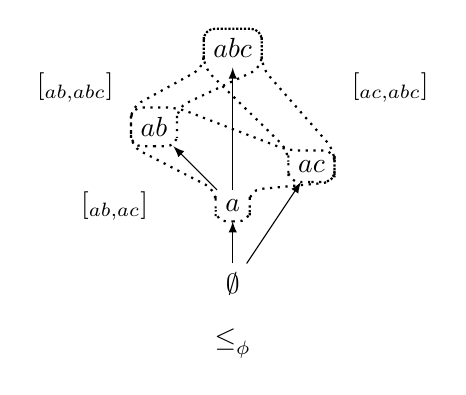
\begin{tikzpicture}
		\node at (0,-0.75){$\le^{\exc}_{\phi}$};
		\node at (0,0)(e){$\emptyset$};
		\node at (0,1)(a){$a$};
		\node at (-1,2)(ab){$ab$};
		\node at (0,3)(abc){$abc$};
		\node at (1,1.5)(ac){$ac$};
		\node at (-2,2.5){$[\px_{ab,abc}]$};
		\node at (2,2.5){$[\px_{ac,abc}]$};
		\node at (-1.5,1){$[\px_{ab,ac}]$};
		\path[-latex] 
		(e) edge (a)
		(a) edge (ab)
		(a) edge (abc)
		(e) edge (ac);
		\draw[thick, dotted, rounded corners=4pt]
			(ab.south)--
			(ab.south east)--
			(ab.east)--
			(ab.north east)--
			(abc.south east)--
			(abc.east)--
			(abc.north east)--
			(abc.north)--
			(abc.north west)--
			(abc.west)--
			(abc.south west)--
			(ab.north west)--
			(ab.west)--
			(ab.south west)--
			(ab.south);
		\draw[thick, dotted, rounded corners=4pt]
			(ac.south)--
			(ac.south east)--
			(ac.east)--
			(ac.north east)--
			(abc.south east)--
			(abc.east)--
			(abc.north east)--
			(abc.north)--
			(abc.north west)--
			(abc.west)--
			(abc.south west)--
			(ac.north west)--
			(ac.west)--
			(ac.south west)--
			(ac.south);
		\draw[thick, dotted, rounded corners=4pt]
			(a.south)--
			(a.south east)--
			(a.east)--
			(a.north east)--
			(ac.south east)--
			(ac.east)--
			(ac.north east)--
			(ac.north)--
			(ac.north west)--
			(ab.north east)--
			(ab.north)--
			(ab.north west)--
			(ab.west)--
			(ab.south west)--
			(a.north west)--
			(a.west)--
			(a.south west)--
			(a.south);
		\end{tikzpicture}
		\caption{
			Exclusive $\re$-revealed preorder $\le^{\exc}_{\phi}$ 
			that is invalidated by postulate $\ppr{\SCON}$,
			even though we would like to see $\le^{\exc}_{\phi}$
			allowed.
		}
		\label{fig:6-hhh-revision-scon-exh-not-good-for-excl}
\end{figure}

\begin{xmpl}{Postulate $\ppr{\SCON}$ does not work for partial preorders}{6-hhh-revision-scon-exh-not-good-for-excl}
	Consider an $\HHH$-revision operator $\re$
	and a Horn formula $\phi$ 
	with $[\phi]=\{\emptyset\}$,
	for which 
	$[\phi\re \px_{ab,abc}]=\{ab,abc\}$,
	$[\phi\re \px_{abc,ac}]=\{abc,ac\}$
	$[\phi\re \px_{ab,ac}]=\{a,ac\}$
	and $\phi\re \px_{\emptyset,w}=\{\emptyset\}$,
	for any interpretation $w$.
	Note that this set of revision results is perfectly consistent 
	with postulates $\ppr{5}$ and $\ppr{7-8}$
	and, furthermore, 
	induces the following exclusive ranking $\le^{\exc}_{\phi}$:
	$ab$, $abc$ and $ac$ are pairwise $\le^{\exc}_{\phi}$-incomparable,
	with the same going for $a$ and $ac$,
	$a<^{\exc}_{\phi}ab$.
	The preorder $\le^{\exc}_{\phi}$ is depicted
	in Figure \ref{fig:6-hhh-revision-scon-exh-not-good-for-excl}.
	This is a legitimate partial preorder, that should be allowed.
	However, under postulate $\ppr{\SCON}$, this setup
	is disallowed.
	Note, we have that: 
	\begin{align*}
		[(\phi\re \px_{ab,abc})\land\px_{ab}]&=\{ab\},\\
		[(\phi\re \px_{abc,ac})\land\px_{abc}]&=\{abc\},\\
		[(\phi\re \px_{ac,ab})\land\px_{ac}]&=\{ac\},\\
		[(\phi\re \px_{ac,ab})\land\px_{ab}]&=\emptyset.
	\end{align*}
	Thus, if we take $w_1 = ab$, $w_2 = abc$ and $w_3 = ac$,
	the setup summarized in Figure \ref{fig:6-hhh-revision-scon-exh-not-good-for-excl}
	would constitute a counter-example to 
	postulate $\ppr{\SCON}$,
	since in this case postulate $\ppr{\SCON}$
	implies that it is not possible to have 
	$(\phi\re \px_{ac,ab})\land\px_{ac}$ consistent
	and 
	$(\phi\re \px_{ac,ab})\land\px_{ab}$ inconsistent.
\end{xmpl}

Example \ref{ex:6-hhh-revision-scon-exh-not-good-for-excl} shows 
that postulate $\ppr{\SCON}$, in conjunction with postulates $\ppr{1-5}$
and $\ppr{7-8}$, leads to unwanted effects, as it eliminates 
preorders that we would like to allow.
Postulate $\ppr{\HSCON}$ is the postulate we need for this case.

That being said, property $\oor{\HSCON}$, which postulate $\ppr{\HSCON}$
guarantees, is still closely connected to Suzumura consistency, which property $\oor{\SCON}$
encodes. In particular, $\oor{\HSCON}$ can be seen as a more specialized version of 
Suzumura consistency, tweaked to work with preorders revealed by $\HHH$-revision operators.
Proposition \ref{prop:6-hhh-revision-HSCON-hscon} shows that, in this context,
property $\oor{\HSCON}$ actually implies Suzumura consistency.

\begin{prp}{}{6-hhh-revision-HSCON-hscon}%
	If $\re$ is an $\HHH$-revision operator that
	satisfies postulates $\ppr{1-5}$ and $\ppr{7-8}$,
	and the exclusive revealed assignment $\as^{\exc}$ satisfies 
	property $\oor{\HSCON}$, then
	$\as^{\exc}$ also satisfies property $\oor{\SCON}$.
\end{prp}
\begin{prf*}{}{}%
	Recall that, in the context of an exclusive revealed assignment $\as^{\exc}$,
	a preference order $\le^{\exc}_{\phi}$ is strict for any distinct interpretations 
	$w_1$ and $w_2$.
	Take, then, pairwise distinct interpretations 
	$w_1$, \dots, $w_n$ such that
	$w_1 <^{\exc}_{\phi}\dots <^{\exc}_{\phi} w_n$
	and suppose,
	in addition, that $w_n <^{\exc}_{\phi} w_1$.
	By the definition of the exclusive revealed 
	assignment, 
	this means that $w_n\in[\phi\re\px_{1,n}]$,
	which, by Lemma \ref{lem:6-hhh-revision-choice-min},
	implies that $w_n\in\min_{\le^{\exc}_{\phi}}\cl_{\horn}(\{w_1,w_n\})$.
	But this contradicts the fact that $\le^{\exc}_{\phi}$
	satisfies property $\oor{\HSCON}$.
\end{prf*}

One of the effects of Proposition \ref{prop:6-hhh-revision-HSCON-hscon}, 
when combined with Theorem \ref{thm:2-suzumura-consistency},
implies that the exclusive revealed preorders 
of an exclusive $\HHH$-revision operator can also be extended
to total preorders on outcomes, as long as the assignment can 
be shown to satisfy property $\oor{\HSCON}$.
For our purposes, though, total preorders are overkill,
since partial preorders are all we are looking for.
Theorem \ref{thm:6-hhh-revision-partial-repr} shows that,
given all the conceptual legwork done so far, 
such partial preorders is within easy reach:
though not exactly the exclusive revealed rankings,
they can be elicited from them by the transitive closure.

\begin{thm}{}{6-hhh-revision-partial-repr}
	An $\HHH$-revision operator $\re$ 
	satisfies postulates $\ppr{1-5}$, $\ppr{7-8}$ (i.e., is exclusive)
	and postulate $\ppr{\HSCON}$
	if and only if there exists
	an $\L_{\horn}$-assignment $\as$ on interpretations
	that 
	satisfies properties $\oor{1-2}$, $\oor{4}$, $\oor{6-7}$ and $\oor{\HC}$
	(i.e., is partial, syntax independent, r-faithful and 
	Horn compliant) 
	and that represents the operator $\re$.
\end{thm}
\begin{prf*}{}{}%
	(``$\Leftarrow$'')
	Take, first, an assignment $\as$ that satisfies the 
	specified conditions.
	Since $\as$ is Horn compliant, this
	implies that the $\as$-induced operator $\re^{\as}$ is an $\HHH$-revision operator.
	Checking that $\re^{\as}$ satisfies postulates $\ppr{1-5}$, $\ppr{7-8}$ is routine.
	Satisfaction of postulate $\ppr{\HSCON}$ 
	follows using Theorem \ref{thm:6-hhh-revision-HSCON-hscon}.

	(``$\Rightarrow$'')
	Take, now, an $\HHH$-revision operator $\re$ that satisfies 
	postulates $\ppr{1-5}$, $\ppr{7-8}$ and $\ppr{\HSCON}$,
	and the $\re$-revealed exclusive $\L_{\horn}$-assignment $\as^{\exc}$.
	If $\phi$ is a Horn formula,
	then the preorder $\le^{\exc}_{\phi}$ is neither complete, nor transitive.
	We know, however, by Theorem \ref{thm:6-hhh-revision-HSCON-hscon},
	that $\le^{\exc}_{\phi}$ satisfies property $\oor{\HSCON}$.

	We take $\le^{\ast}_{\phi}$ to be the transitive 
	and reflexive closure of $\le^{\exc}_{\phi}$,
	and the assignment $\as^{\ast}$ to be defined by $\as^{\ast}\!\!(\phi) \defeq \le^{\ast}_{\phi}$.
	We show, now, that $\as^{\ast}$ is the assignment we are looking for.
	We have that $\as^{\ast}$ is reflexive and transitive by definition,
	and using postulate $\ppr{2}$ it can be shown in the usual way that $\as^{\ast}$ is r-faithful.
	The only thing left to be shown is that $\as^{\ast}$ represents $\re$,
	i.e., that $[\phi\re\mu]=\min_{\le^{\ast}_{\phi}}[\mu]$.
	We show this by double inclusion.

	(``$\subseteq$'')
	Take $w\in[\phi\re\mu]$ and suppose $w\notin\min_{\le^{\ast}_{\phi}}[\mu]$.
	This means that there exists $w'\in[\mu]$ such that $w'<^{\ast}_{\phi}w$,
	i.e., that there exist pairwise distinct interpretations 
	$w_0$, \dots, $w_k$ such that:
	$$
		w'<^{\exc}_{\phi} w_0<^{\exc}_{\phi}\dots <^{\exc}_{\phi}w_k <^{\exc}_{\phi} w.
	$$
	Since $\le^{\exc}_{\phi}$ satisfies property $\oor{\HSCON}$,
	it follows that $w\notin\min_{\le^{\exc}_{\phi}}\cl_{\horn}(\{w_1,w_n\})$.
	At the same time, we have that:
	\begin{align*}
		(\phi\re\mu)\land\px_{w,w'}&\models \phi\re(\mu\land\px_{w,w'}) &\text{by}~\ppr{5}\\
										&\equiv \phi\re\px_{w,w'}. &\text{by}~\ppr{4}
	\end{align*}
	Since $w\in[\phi\re\mu]$, this implies that $w\in[\phi\re\px_{w,w'}]$
	and,
	using Lemma \ref{lem:6-hhh-revision-choice-min}
	we conclude that $w \in\min_{\le^{\exc}_{\phi}}\cl_{\horn}(\{w_1,w_n\})$,
	which creates a contradiction.

	(``$\supseteq$'')
	Take $w\in\min_{\le^{\ast}_{\phi}}[\mu]$ and an arbitrary interpretation 
	$w'\in[\mu]$. We will show first that $w\in[\phi\re\px_{w,w'}]$.
	Suppose that $w\notin[\phi\re\px_{w,w'}]$.
	Since $[\px_{w,w'}]=\cl_{\horn}(\{w,w'\})$,
	there are two relevant cases to look at.

	\emph{Case 1}.
	If $[\phi\re\px_{w,w'}]=\{w'\}$ or $[\phi\re\px_{w,w'}]=\{w',w\cap w'\}$,
	then, by the definition of $\le^{\exc}_{\phi}$
	it follows that $w'<^{\exc}_{\phi}w$,
	which implies that $w'<^{\ast}_{\phi}w$,
	contradicting the fact that $w\in\min_{\le^{\ast}_{\phi}}[\mu]$.

	\emph{Case 2}.
	If $[\phi\re\px_{w,w'}]=\{w\cap w'\}$, then we have that:
	\begin{align*}
		\phi\re\px_{w,w\cap w'} &\models \px_{w,w'},\\
		\phi\re\px_{w,w'} &\models \px_{w,w\cap w'}.
	\end{align*}
	Using postulate $\ppr{7}$, 
	it follows that 
	$\phi\re\px_{w,w\cap w'}\equiv \phi\re\px_{w,w'}$,
	i.e., $[\phi\re\px_{w,w\cap w'}]=\{w\cap w'\}$.
	This, now, implies that $(w\cap w')<^{\exc}_{\phi} w$,
	from which it follows that $(w\cap w')<^{\ast}_{\phi}w$.
	Since $w\in[\mu]$, $w'\in[\mu]$
	and the fact that $\mu$ is a Horn formula and 
	thus $[\mu]$ is closed under intersection, 
	we infer that $(w\cap w')\in[\mu]$ as well.
	But this, together with the previously inferred 
	statement that $(w\cap w')<^{\ast}_{\phi}w$,
	contradicts the fact that $w\in\min_{\le^{\ast}_{\phi}}[\mu]$.
	We conclude, therefore, that $w\in[\phi\re\px_{w,w'}]$.

	For the final step, we use postulate $\ppr{8}$
	and the fact that $\mu=\bigvee_{w'\in[\mu]}\px_{w,w'}$
	to conclude that $w\in[\phi\re(\bigvee_{w'\in[\mu]}\px_{w,w'})]$.
\end{prf*}

Theorem \ref{thm:6-hhh-revision-partial-repr} shows that 
partial preorders can be used to represent exclusive 
$\HHH$-revision operators, just like total preorders can be used to 
represent exhaustive $\HHH$-revision operators.
In doing so, some additions need to be made, both on the semantic side
and on the syntactic side. Firstly, Horn compliance 
works with both total and partial preorders, and guarantees that 
revision always falls within the Horn fragment.
Then, Suzumura consistency, together with its accompanying postulate,
kicks in to make sure that the revealed assignments do not contain cycles
or other unwanted side effects. Interestingly, Suzumura consistency needs 
to be slightly modified in order to work for partial preorders and postulates 
$\ppr{1-5}$ and $\ppr{7-8}$.









\section{Horn update by Horn formulas}\label{sec:6-hhh-update}
All the wisdom gained in Section \ref{sec:6-hhh-revision} can be put to 
use to understand update with Horn formulas,
and this section is dedicated to spelling out the details.
Since the primary plot points for Horn update are the same as for Horn revision with 
Horn formulas, we defer to the previous section for discussion and motivation.

An \emph{$\HHH$-update operator $\up$} is a function  
$\up\colon\L_{\horn}\times\L_{\horn}\rightarrow\L_{\horn}$,
taking as input two Horn formulas, 
typically denoted by $\phi$ and $\mu$
and referred to as the prior and new information, respectively,
and returning a Horn formula,
typically denoted by $\phi\up\mu$
and referred to as the posterior updated information.
The postulates for $\HHH$-update revision
are the standard update postulates $\ppu{1-9}$
as presented in Section \ref{sec:3-update},
and particularized, as for revision, to Horn formulas.
The postulates are expected to 
apply to any Horn formulas
$\phi$, $\phi_{1}$, $\phi_{2}$,
$\mu$, $\mu_{1}$ and $\mu_{2}$
and complete Horn formulas $\dot{\phi}$:

\begin{description}
	\item[($\ppu{1}$)] $\phi\up\mu\models\mu$.	
	\item[($\ppu{2}$)] If $\phi\models\mu$, then $\phi\up\mu\equiv\phi$.
	\item[($\ppu{3}$)] If $\phi$ and $\mu$ are consistent, 
		then $\phi\up\mu$ is consistent.
	\item[($\ppu{4}$)] If $\phi_1\equiv\phi_2$ and $\mu_1\equiv\mu_2$, 
		then $\phi_1\up\mu_1\equiv\phi_2\up\mu_2$.
	\item[($\ppu{5}$)] $(\phi\up\mu_1)\land\mu_2\models\phi\up(\mu_1\land\mu_2)$.
	\item[($\ppu{6}$)] If $(\dot{\phi}\up\mu_1)\land\mu_2$ is consistent, 
		then $\dot{\phi}\up(\mu_1\land\mu_2)\models(\dot{\phi}\up\mu_1)\land\mu_2$.
	\item[($\ppu{7}$)] If $\phi\up\mu_1\models\mu_2$ and $\phi\up\mu_2\models\mu_1$, 
		then $\phi\up\mu_1\equiv\phi\up\mu_2$
	\item[($\ppu{8}$)] If $\mu\equiv \mu_{1}\lor\mu_{2}$.
		then $(\dot{\phi}\up\mu_1)\land(\dot{\phi}\up\mu_2)\models\dot{\phi}\up\mu$.
	\item[($\ppu{9}$)] If $\phi\equiv\phi_1\lor\phi_2$,
		then $(\phi_{1}\lor\phi_{2})\up\mu\equiv(\phi_1\up\mu)\lor(\phi_2\up\mu)$.
\end{description}

As for $\L$-update, we are more interested in the variant of postulate
$\ppu{9}$ presented below.
Since we are working in the Horn fragment, 
this means that proxies are intended to be Horn formulas:
in other words, if $v$ is an interpretations, then 
$\px_{v}$ is an $\L_{\horn}$-proxy of $\{v\}$,
i.e., a Horn formula such that $[\px_{v}]=\cl_{\horn}(\{v\})=\{v\}$.

\begin{description}
	\item[($\ppu{10}$)] $\phi\up\mu\equiv \bigvee_{v\in[\phi]}(\px_{v}\up\mu)$.
\end{description}

Postulate $\ppu{10}$ is equivalent to postulate $\ppu{9}$ 
even when applied to Horn formulas, 
and says that $\phi\up\mu$ can be decomposed
in the results for $\px_{v}\up\mu$, for every $v\in[\phi]$.

On the semantic side we can use, as for $\L$-update, 
assignments on complete formulas: every complete formula is,
or can be thought of, as a Horn formula, 
in the sense that its set of models is $\horn$-closed.
Thus, we can work here with n \emph{$\L_{\comp}$ assignment $\as$ on interpretations}, 
which is a function $\as\colon\L_{\comp}\rightarrow 2^{\U\times\U}$,
taking as input a complete formula $\dot{\phi}$ and returning
a binary relation on interpretations.
The properties we are interested in are as follows, 
for any complete Horn propositional formulas $\dot{\phi}$, $\dot{\phi_{1}}$, $\dot{\phi_{2}}$
and interpretations $w$, $v$, $w_1$ and $w_2$:

\begin{description}
	\item[($\oou{1}$)] $w\le_{\dot{\phi}} w$.
	\item[($\oou{2}$)] If $w_1\le_{\dot{\phi}} w_2$ and $w_2\le_{\dot{\phi}} w_3$, 
		then $w_1\le_{\dot{\phi}} w_3$.
	\item[($\oou{3}$)] $w_1\le_{\dot{\phi}} w_2$ or $w_2\le_{\dot{\phi}} w_1$.
	\item[($\oou{4}$)] If $\dot{\phi_1}\equiv \dot{\phi_2}$, then $\le_{\dot{\phi_1}} = \le_{\dot{\phi_2}}$. 
	\item[($\oou{5}$)] If $[\dot{\phi}]=\{v\}$ and $w\neq v$, then $v<_{\dot{\phi}} w$.
\end{description}

As usual, an $\L_{\comp}$-assignment $\as$ on interpretations is 
\emph{partial} if it satisfies properties $\oou{1-2}$,
\emph{total} if it satisfies properties $\oou{1-3}$,
\emph{syntax insensitive} if it satisfies property $\oou{4}$
and \emph{u-faithful} if it satisfies property $\oou{5}$.

If $\up$ is an $\HHH$-update operator and 
$\as$ is an $\L_{\comp}$-assignment on interpretations,
then \emph{$\as$ represents $\up$}
(and \emph{$\up$ is represented by $\as$})
if, for any Horn formulas $\phi$ and $\mu$,
it holds that $[\phi\up\mu] = \bigcup_{v\in[\phi]}\min_{\le_{\px_{v}}}[\mu]$. 
Given an $\L_{\comp}$-assignment $\as$ on interpretations, 
the \emph{$\as$-induced $\L$-update operator $\re^\as$} is defined,
for any Horn formulas $\phi$ and $\mu$, 
by taking:
$$
	[\phi\up^\as\mu]\defeq\bigcup_{v\in[\phi]}\min_{\le_{\px_{v}}}[\mu].
$$
If $\up$ is an $\HHH$-update operator and $\dot{\phi}$ is a complete (Horn) formula,
the \emph{exhaustive $\up$-revealed plausibility relation $\le^\exh_{\dot{\phi}}$} 
and the \emph{exclusive $\up$-revealed plausibility relation $\le^\exc_{\dot{\phi}}$} 
are defined, for any interpretations $w_1$ and $w_2$, respectively, as:
\begin{align*}
	w_1\le^\exh_{\dot{\phi}} w_2 &~\text{if}~w_1\in[{\dot{\phi}}\up\px_{1,2}],\\
	w_1\le^\exc_{\dot{\phi}} w_2 &~\text{if either}~w_1=w_2,
			\text{or}~w_1\in[{\dot{\phi}}\up\px_{1,2}]~\text{and}~w_2\notin[{\dot{\phi}}\up\px_{1,2}].
\end{align*}
The \emph{exhaustive $\up$-revealed $\L_{\comp}$-assignment $\as^\exh$} 
and \emph{exclusive $\up$-revealed $\L_{\comp}$-assignment $\as^\exc$} 
are obtained by taking $\as^\exh\!\!(\dot{\phi})=\le^\exh_{\dot{\phi}}$ 
and $\as^\exc\!\!(\dot{\phi})=\le^\exc_{\dot{\phi}}$, for any complete 
Horn formula $\dot{\phi}$.
As for revision,
$\up^{\as}$ is defined as an $\L$-update operator,
i.e., an operator that returns propositional formulas and
not necessarily Horn formula,
because an assignment needs to be restricted if it is to deliver 
results compatible with the Horn fragment.

Since update becomes indistinguishable from revision when $\phi$
is complete, the same problems that plague $\HHH$-revision also occur 
when working with $\HHH$-update operators.
Note, for instance, that the prior information in 
Examples \ref{ex:6-hhh-revision-standard-ops-no-good} is complete:
this shows that this example is relevant to $\HHH$-update as well 
and, in particular, that existing update operators, such as Forbus and Winslett's
operators do not work as $\HHH$-update operators.
The solution, of course, is to restrict the assignments we are working with 
using a property that, 
as we might expect, is a version of Horn compliance adapted to the context 
of update.
This property says that the following must hold,
for any Horn formulas $\phi$ and $\mu$:

\begin{description}
	\item[($\oou{\HC}$)] $\bigcup_{v\in[\phi]}\min_{\le_{\px_{v}}}[\mu]$ is $\horn$-closed.
\end{description}


% This property applies for any interpretations $w_1$, $w_2$
% and complete Horn formulas $\dot{\phi_{1}}$ and $\dot{\phi_{2}}$:

% \begin{description}
% 	\item[($\oou{\dTCMPL}$)] If $w_1 \not<_{\dot{\phi}}w_2$ and $w_2\not<_{\dot{\phi}}w_1$, 
% 		then there exists a complete formula $\dot{\phi_{3}}$ such that		
% 		$(w_1\cap w_2) \in\min_{\le_{\dot{\phi_{3}}}}\cl_{\horn}(\{w_1,w_2\})$.
% \end{description}

Property $\oou{\HC}$, 
where `$\HC$' stands for \emph{Horn compliance},
works along the same lines as Horn compliance 
in the context of $\HHH$-revision \cite{DelgrandeP15},
and ensures that the $\as$-induced update operator 
is an $\HHH$-update operator.



% As with property $\oor{\TCMPL}$, the goal of property $\oou{\dTCMPL}$
% is to ensure that a $\L_{\comp}$-assignment on interpretations
% can represent an $\HHH$-update operator.

% \begin{thm}{}{6-hhh-update-dTCMPL-well-defined}
% 	If $\up$ is an $\L$-update operator
% 	and $\as$ is an $\L_{\comp}$-assignment on interpretations
% 	that represents it,
% 	then $\up$ is an $\HHH$-update operator, 
% 	when restricted to Horn formulas,
% 	if and only if $\up$ satisfies property $\oou{\dTCMPL}$,
% 	when restricted to Horn formulas.
% \end{thm}
% \begin{prf*}{}{}%
	
% \end{prf*}

Furthermore, Examples \ref{ex:6-hhh-revision-cycles} and \ref{ex:6-hhh-revision-scon-exh-not-good-for-excl}
can also be adapted to $\HHH$-update operator, 
showing that the standard postulates do not exclude unwanted assignments.
The fixes, as for $\HHH$-revision, involve 
a series of semantic properties on the revealed preference orders,
coupled with corresponding logical postulates.
The semantic properties are intended to apply for any 
complete Horn formulas $\dot{\phi}$
and interpretations $w_1$, \dots, $w_n$, and are as follows:

\begin{description}
	\item[($\oou{\SCON}$)] If $w_1 \le_{\dot{\phi}}\dots \le_{\dot{\phi}}w_n$,
	then $w_{n}\not<_{\dot{\phi}} w_{1}$.
	\item[($\oou{\HSCON}$)] If $w_1 <_{\dot{\phi}}\dots <_{\dot{\phi}} w_n$,
	then $w_n\notin\min_{\le_{\dot{\phi}}}\cl_{\horn}(\{w_1,w_n\})$.
\end{description}

These properties are equivalent to properties $\oor{\SCON}$ and $\oor{\HSCON}$,
with the only difference being that they are particularized to complete Horn formulas.
As expected, property $\oou{\SCON}$ is expected to hold for the exhaustive 
revealed assignment and $\oou{\HSCON}$ is intended to hold for the exclusive 
revealed assignment.

On the syntactic side 
we use the following postulates,
or more precesily postulate schemas,
intended to work for any complete Horn formulas $\dot{\phi}$,
interpretations $w_1$, \dots, $w_n$
and the corresponding $\L_{\horn}$-proxies:

\begin{description}
	\item[($\ppu{\SCON}$)]
	If $(\dot{\phi}\up\px_{1,2})\land\px_{1}$ is consistent,
		\dots,
		$(\dot{\phi}\up\px_{n-1,n})\land\px_{n-1}$ is consistent,
	then it does not hold both that
	$(\dot{\phi}\up\px_{n,1})\land\px_{n}$ is consistent
	and that $(\dot{\phi}\up\px_{n,1})\land\px_{1}$ is inconsistent.

	\item[($\ppu{\HSCON}$)]
	If 
		$(\dot{\phi}\up\px_{1,2})\land\px_{1}$ is consistent and
		$(\dot{\phi}\up\px_{1,2})\land\px_{2}$ is inconsistent,
		\dots,
		$(\dot{\phi}\up\px_{n-1,n})\land\px_{n-1}$ is consistent and
		$(\dot{\phi}\up\px_{n-1,n})\land\px_{n}$ is inconsistent,
	then $(\dot{\phi}\up\px_{n,1})\land\px_{n}$ is inconsistent.
\end{description}

Postulates $\ppu{\SCON}$ and $\ppu{\HSCON}$ are direct rewritings of postulates 
$\ppr{\SCON}$ and $\ppr{\HSCON}$ from $\HHH$-revision,
and the argument that they go hand in hand with propeerties $\oou{\SCON}$ and $\oou{\HSCON}$
is entirely similar.

With most of the theoretical groundwork having been laid in Section \ref{sec:6-hhh-revision},
the representation results can be stated now in quick succession.
The first result concerns $\HHH$-update operators that satisfy postulates $\ppu{1-6}$, $\ppu{9}$
and $\ppu{\SCON}$, and are represented using total assignments.

\begin{thm}{}{6-hhh-update-repr-total}
	An $\HHH$-update operator $\up$ 
	satisfies postulates $\ppu{1-6}$, $\ppu{9}$ and $\ppu{\SCON}$
	if and only if there exists
	an $\L_{\comp}$-assignment $\as$ on interpretations
	that satisfies properties $\oou{1-5}$ and $\oou{\HC}$
	(i.e., is total, syntax independent, u-faithful and Horn compliant)
	and that represents the operator $\up$.
\end{thm}
\begin{prf*}{}{}%
	Horn compliance of $\as$ guarantees that the $\as$-induced update operator $\up^{\as}$ 
	is an $\HHH$-update operator, and showing that $\up^{\as}$ satisfies postulates 
	$\ppu{1-6}$, $\ppu{9}$ and $\ppu{\SCON}$ is straightforward, and works in the same way 
	as for $\HHH$-revision operators.
	Conversely, if $\up$ satisfies postulates $\ppu{1-6}$, $\ppu{9}$ and $\ppu{\SCON}$,
	then we use the argument for $\HHH$-revision operators that satisfy postulates $\ppr{1-6}$,
	particularized to complete formulas.
	That is to say, using Theorem \ref{thm:6-hhh-revision-total-repr},
	we know that the $\up$-revealed exhaustive assignment represents $\up$ for the case of complete formulas,
	i.e., if $\dot{\phi}$ is a complete Horn formula,
	then $[\dot{\phi}\up\mu]=\min_{\le_{\dot{\phi}}}[\mu]$, for any Horn formula $\mu$.
	We now use postulate $\ppu{9}$ to extend this to the fact that 
	$[\phi\up\mu]=\bigcup_{v\in[\phi]}\min_{\le_{\px_{v}}}[\mu]$,
	for any Horn formula $\phi$.
	This shows that $\as^{\exh}$ represents the operator $\up$.
\end{prf*}

Accompanying this result is, of course, a result for 
$\HHH$-update operators that satisfy postulates $\ppu{1-5}$, $\ppu{7-8}$, $\ppu{9}$
and $\ppu{\HSCON}$, and are represented using partial assignments.

\begin{thm}{}{6-hhh-update-repr-partial}
	An $\HHH$-update operator $\up$ 
	satisfies postulates $\ppu{1-5}$, $\ppu{7-8}$, $\ppu{9}$ and $\ppu{\HSCON}$
	if and only if there exists
	an $\L_{\comp}$-assignment $\as$ on interpretations
	that satisfies properties $\oou{1-2}$, $\oou{4-5}$ and $\oou{\HC}$
	(i.e., is partial, syntax independent, u-faithful and Horn compliant)
	and that represents the operator $\up$.
\end{thm}
\begin{prf*}{}{}%
	The proof here follows the same lines as the proof for Theorem \ref{thm:6-hhh-update-repr-total},
	but using the results in Theorem \ref{thm:6-hhh-revision-partial-repr} to construct the 
	revealed assignment that ends up representing the operator $\up$.
\end{prf*}

Theorems \ref{thm:6-hhh-update-repr-total} and \ref{thm:6-hhh-update-repr-partial}
are straightforward applications of Theorems \ref{thm:6-hhh-revision-total-repr} 
and \ref{thm:6-hhh-revision-partial-repr}, but the insights gained in making these results 
work show that they are robust enough to function across different contexts.


























\section{Related work}\label{sec:6-rw}
Work on belief change for the Horn fragment began with 
work on contraction \cite{Delgrande08,DelgrandeW10,DelgrandeW13}, 
the conclusions of which, however, were that traditional AGM techniques,
such as ones based on remainder sets, did not work as expected
in the Horn fragment. Alternative constructions were proposed,
e.g., in terms of \emph{weak remainder sets}, which were later taken 
up and extended \cite{BoothMV09,BoothMVW11,ZhuangP14}.

Getting Horn contraction right is important for revision as well,
since contraction and revision are traditionally thought to be inter-definable
via the Levi and Harper identities \cite{Levi91,Harper76}.
However, these identities involve negations and, since the negation of a Horn formula
is not necessarily a Horn formula, their application to the Horn fragment is limited
\cite{Delgrande08,ZhuangPZ13,ZhuangPZ17}.

Thus, it seems that Horn revision is best thought of on its own.
In this, some of the most promising approaches to revision of Horn formulas 
have been model based: given our understanding of revision 
as a choice function on outcomes, this line of research is particularly apposite.
Indeed, our starting point has been the model developed originally 
by James Delgrande and Pavlos Peppas \cite{DelgrandeP15,DelgrandePW18},
which we have sought to emulate here using 
partial preorders and weaker versions of the classical postulates.
Our understanding of this model and its variations is thoroughly semantic, with the main 
actors, and guarantors of rationality, being the preorders on interpretations:
in our view, as long as we are able to get the right kinds of preorders 
(i.e., transitive, or at least non-cyclic), then we are on the right track.
In this light, the role of the additional postulates is to make sure 
that the preorders behave well: it is difficult to justify a postulate 
such as $\ppr{\SCON}$ or $\ppr{\HSCON}$ other than by appeal to the 
semantic property it induces. This is also why we choose to 
formulate these postulates using $\L_{\horn}$-proxies 
(i.e., as choices over pairs of interpretations)
rather than by using generic Horn formulas, as in \cite{DelgrandeP15,DelgrandePW18}.

This preorder-led view is also what led us to the rational choice literature,
where the relationship between choice functions and various types of preference 
relations has been a mainstay since the very early days. 
Suzumura consistency \cite{Suzumura76,Suzumura83,BossertS10} 
jumped out as the most obvious connecting element, but the rational choice literature 
is awash in distinctions and properties that could be useful to belief change as well. 
For instance, the acyclicity postulate presented in \cite{DelgrandeP15,DelgrandePW18}
occurs in an equivalent formulation in rational choice theory, as the 
\emph{Strong Axiom of Revealed Preference (SARP)} \cite{Hansson68,Suzumura16}.

Belief change in the Horn fragment, as we have seen, is caught in between 
two equally demanding requirements: one is the normative demands 
provided by the postulates,
i.e., the requirement that the revision operator should satisfy a set 
of desirable properties;
the other is the expressibility requirement,
i.e., we need to make sure that the result 
can be expressed as a Horn formula. 
In this chapter we have typically opted to hold fast to the postulates, and even 
complement them if needed, but this has had the effect of limiting the range 
of available operators: none of the tried and tested revision or update operators 
works in the Horn fragment. 
A different approach is to take the existing operators and repair their output when 
it does not fit into the Horn fragment, e.g., by taking the $\horn$-closure of 
the selected set of interpretations as the result. 
The advantage of this method is that it is guaranteed to produce $\horn$-closed
results; the disadvantage is that some of the postulates might not be satisfied 
\cite{CreignouPPW14,CreignouPRW16,CreignouKP18}.

It should also be mentioned that belief change in fragments is not 
confined to contraction and revision (or update), 
with existing work on merging in the Horn fragment
\cite{HaretRW15,HaretRW17},
and the Horn fragment is not the 
only formalism of interest,
with logic programs, Answer Set Programs and Description Logics 
all enjoying their own fifteen minutes of AGM fame
\cite{DelgrandeW13,ZhuangWWQ16,BinnewiesZWS18,ZhuangWWD19,ZheleznyakovKNC20}.










\section{Conclusion}\label{sec:6-conclusion}
In this chapter we have looked at revision of Horn formulas 
using both propositional and Horn formulas:
though the results have ultimately taken a familiar form
(i.e., as representation theorems),
the overall work surrounding them shows that restricting the 
language in which belief change occurs does not allow us 
to seamlessly derive the same conclusions.

Over and over, we have seen that the standard postulates 
do not generalize immediately to the Horn fragment.
For revision with propositional formulas, 
the standard postulate $\ppr{2}$ becomes problematic and 
the newly introduced neutrality postulate $\ppr{\NEUT}$
proves impossible to satisfy.
For revision, as well as update, with Horn formulas,
it is postulates $\ppr{5-6}$, and, respectively, $\ppu{5-6}$,
that end up being less powerful at forcing the assignments 
into the right shape.
The solution, we have seen, has been to complement the standard 
postulates by new ones: typically, a special postulate depending 
on whether we were working with total or partial preorders.
In doing so, we extended existing work on revision in the Horn fragment 
\cite{DelgrandeP15,DelgrandePW18},
and revealed some interesting principles that underlie belief change in fragments.

Lemma \ref{lem:6-hhh-revision-choice-min}, in particular, 
is interesting enough that it deserves more consideration:
in essence, it says that if a chain of comparisons 
favors an interpretation $w_1$ over $w_n$, then $w_n$ should not 
be chosen over $w_1$  when the choice 
is over the proxy of $w_1$ and $w_n$.
This property holds for all the settings we have encountered so far 
(total and partial orders, propositional logic as well as its Horn fragment),
but it was only for the Horn fragment with partial preorders that we had 
to spell it out explicitly.
As such, Lemma \ref{lem:6-hhh-revision-choice-min} captures a property that
is likely to prove important for belief change in formalisms other than
propositional logic and the Horn fragment.







